%%%%
% Modificación de una plantilla de Latex para adaptarla al castellano.
%%%

%%%%%%%%%%%%%%%%%%%%%%%%%%%%%%%%%%%%%%%%%
% Thin Sectioned Essay
% LaTeX Template
% Version 1.0 (3/8/13)
%
% This template has been downloaded from:
% http://www.LaTeXTemplates.com
%
% Original Author:
% Nicolas Diaz (nsdiaz@uc.cl) with extensive modifications by:
% Vel (vel@latextemplates.com)
%
% License:
% CC BY-NC-SA 3.0 (http://creativecommons.org/licenses/by-nc-sa/3.0/)
%
%%%%%%%%%%%%%%%%%%%%%%%%%%%%%%%%%%%%%%%%%

%----------------------------------------------------------------------------------------
%	PACKAGES AND OTHER DOCUMENT CONFIGURATIONS
%----------------------------------------------------------------------------------------

\documentclass[a4paper, 11pt]{article} % Font size (can be 10pt, 11pt or 12pt) and paper size (remove a4paper for US letter paper)

\usepackage[protrusion=true,expansion=true]{microtype} % Better typography
\usepackage{graphicx} % Required for including pictures
\usepackage[usenames,dvipsnames]{color} % Coloring code
\usepackage{wrapfig} % Allows in-line images
\usepackage[utf8]{inputenc}

% Imágenes
\usepackage{graphicx} 

\usepackage{amsmath}
% para importar svg
%\usepackage[generate=all]{svgfig}

% sudo apt-get install texlive-lang-spanish
\usepackage[spanish]{babel} % English language/hyphenation
\selectlanguage{spanish}
% Hay que pelearse con babel-spanish para el alineamiento del punto decimal
\decimalpoint
\usepackage{dcolumn}
\newcolumntype{d}[1]{D{.}{\esperiod}{#1}}
\makeatletter
\addto\shorthandsspanish{\let\esperiod\es@period@code}
\makeatother

\usepackage{longtable}
\usepackage{tabu}
\usepackage{supertabular}

\usepackage{multicol}
\newsavebox\ltmcbox

% Para algoritmos
\usepackage{algorithm}
\usepackage{algorithmic}
\usepackage{amsthm}
\floatname{algorithm}{Algoritmo}
\renewcommand{\listalgorithmname}{Lista de algoritmos}
\renewcommand{\algorithmicrequire}{\textbf{Entrada:}}
\renewcommand{\algorithmicensure}{\textbf{Salida:}}
\renewcommand{\algorithmicend}{\textbf{fin}}
\renewcommand{\algorithmicif}{\textbf{si}}
\renewcommand{\algorithmicthen}{\textbf{entonces}}
\renewcommand{\algorithmicelse}{\textbf{en otro caso}}
\renewcommand{\algorithmicelsif}{\algorithmicelse,\ \algorithmicif}
\renewcommand{\algorithmicendif}{\algorithmicend\ \algorithmicif}
\renewcommand{\algorithmicfor}{\textbf{para }}
\renewcommand{\algorithmicforall}{\textbf{para cada}}
\renewcommand{\algorithmicdo}{\textbf{}}
\renewcommand{\algorithmicendfor}{\algorithmicend\ \algorithmicfor}
\renewcommand{\algorithmicwhile}{\textbf{mientras}}
\renewcommand{\algorithmicendwhile}{\algorithmicend\ \algorithmicwhile}
\renewcommand{\algorithmicloop}{\textbf{repetir}}
\renewcommand{\algorithmicendloop}{\algorithmicend\ \algorithmicloop}
\renewcommand{\algorithmicrepeat}{\textbf{repetir}}
\renewcommand{\algorithmicuntil}{\textbf{hasta que}}
\renewcommand{\algorithmicprint}{\textbf{imprimir}} 
\renewcommand{\algorithmicreturn}{\textbf{devolver}} 
\renewcommand{\algorithmictrue}{\textbf{true }} 
\renewcommand{\algorithmicfalse}{\textbf{false }} 
\renewcommand{\algorithmicand}{\textbf{y}}
\renewcommand{\algorithmicor}{\textbf{o}}


% Para matrices
\usepackage{amsmath}

% Símbolos matemáticos
\usepackage{amssymb}
\let\oldemptyset\emptyset
\let\emptyset\varnothing

\usepackage[section]{placeins} % Para gráficas en su sección.
\usepackage{mathpazo} % Use the Palatino font
\usepackage[T1]{fontenc} % Required for accented characters
\newenvironment{allintypewriter}{\ttfamily}{\par}
\setlength{\parindent}{0pt}
\parskip=8pt
\linespread{1.05} % Change line spacing here, Palatino benefits from a slight increase by default

\makeatletter
\renewcommand\@biblabel[1]{\textbf{#1.}} % Change the square brackets for each bibliography item from '[1]' to '1.'
\renewcommand{\@listI}{\itemsep=0pt} % Reduce the space between items in the itemize and enumerate environments and the bibliography
\newcommand{\imagen}[2]{\begin{center} \includegraphics[width=90mm]{#1} \\#2 \end{center}}

\renewcommand{\maketitle}{ % Customize the title - do not edit title and author name here, see the TITLE block below
\begin{flushright} % Right align
{\LARGE\@title} % Increase the font size of the title

\vspace{50pt} % Some vertical space between the title and author name

{\large\@author} % Author name
\\\@date % Date

\vspace{40pt} % Some vertical space between the author block and abstract
\end{flushright}
}


%Basado en: http://en.wikibooks.org/wiki/LaTeX/Theorems
\usepackage{amsthm}
\newtheorem*{mydef}{Definición}
\newtheorem{mydefn}{Definición}
\newtheorem{theorem}{Teorema}
\everymath{\displaystyle} % Displaystyle por defecto

%----------------------------------------------------------------------------------------
%	TITLE
%----------------------------------------------------------------------------------------

\title{\textbf{Práctica 3}\\ % Title
Algoritmos Greedy} % Subtitle

\author{\textsc{Óscar Bermúdez,\\Francisco David Charte,\\Ignacio Cordón,\\José Carlos Entrena,\\Mario Román} % Author
\\{\textit{Universidad de Granada}}} % Institution

\date{\today} % Date

%----------------------------------------------------------------------------------------

\begin{document}

\maketitle % Print the title section

\renewcommand{\abstractname}{Resumen} % Uncomment to change the name of the abstract to something else
\begin{abstract}
\end{abstract}
{\parskip=2pt
\tableofcontents
}
\pagebreak


\section{Terminales de venta}
El problema de los terminales de venta consiste en, dada una cantidad de dinero, conseguir el mínimo número de monedas posible para devolverlo al cliente.
Diseñar un algoritmo Greedy que resuelva esta situación es sencillo, dados los siguientes valores de las monedas de euro: 0.01, 0.02, 0.05, 0.10, 0.20, 0.50 y 1 euro.
\subsection{Algoritmo}
La técnica que se seguirá es ir escogiendo la mayor cantidad de monedas del mayor valor posible sin superar la cantidad de dinero restante a cada momento:

\begin{algorithm}[H]
	\begin{algorithmic}[1]
		\REQUIRE \ \\
        	\texttt{monedas}, vector con los valores de monedas disponibles \\
        	\texttt{precio}, cantidad de dinero a devolver\\\
     	\STATE{Ordenar \texttt{monedas} de mayor a menor}
     	%  He usado un vector aunque en el código final usábamos 
     	%  un diccionario, si queréis lo cambio -David
     	\STATE{Crear un vector \texttt{vuelta}}
		\FORALL{\texttt{moneda} en \texttt{monedas}}
			\STATE{\texttt{cantidad} $\gets$ \texttt{precio} / \texttt{moneda}}
			\STATE{\texttt{precio} $\gets$ \texttt{precio} $-$ \texttt{cantidad} $\times$ \texttt{moneda}}
			\STATE{Añadir [\texttt{moneda}, \texttt{cantidad}] a \texttt{vuelta}}
		\ENDFOR
		\RETURN{vuelta}
	\end{algorithmic}
    \caption{Devolución en mínimo número de monedas}
    \label{monedas}
\end{algorithm}  

\subsection{Contraejemplo}
El buen funcionamiento del algoritmo dependerá de los valores de posibles monedas que se utilicen. En el ejemplo de los sellos de valores 0.54, 0.32, 0.17 y 0.01 euros,
habrá casos en los que el algoritmo no consiga el mínimo número de monedas. Por ejemplo, si queremos obtener un valor de 0.34 euros:
\begin{itemize}
	\item Solución del algoritmo: 0.32 + 0.01 + 0.01 (3 sellos)
	\item Solución óptima: 0.17 + 0.17 (2 sellos)
\end{itemize}

Esto se debe a que hay valores de sellos cuyo doble es mayor que otro valor, es decir, con dos sellos de 0.17 se consiguen 34 céntimos, que es mayor que otro sello existente superior al de 17, el sello de 32 céntimos. Esto provoca que el algoritmo escoja un sello de mayor valor de forma equivocada, ya que con dos sellos de menor valor se reduce más la distancia al objetivo, pudiendo llegar a una solución mejor.
  
\section{Red de comunicaciones}
  \subsection{Algoritmo}
    Dado un conjunto de ciudades, buscamos interconectarlas con una red que minimice la longitud de red. 
    Modelizaremos el problema como un grafo completo $G$ del conjunto de ciudades $E$. Con aristas 
    $V = \left\{ [a,b] |\ a,b \in E \right\}$, donde la arista conectando los nodos $a$ y $b$ tiene peso 
    igual a la distancia que los separa:

    \begin{equation}
     \forall [a,b]\in V:\quad  w([a,b]) = dist (a,b)
    \end{equation}

    Pretendemos interconectar ciudades de manera que la suma total de las distancias de los caminos hechos 
    sea mínima. Es decir, buscamos el subgrafo recubridor de menor peso. Como un grafo recubridor con ciclos 
    tiene siempre un subgrafo recubridor estrictamente contenido en él, buscamos sólo entre los grafos acíclicos.
    El subgrafo acíclico recubridor de menor costo es el árbol recubridor minimal. Es decir, buscamos el árbol
    recubridor minimal euclídeo de un conjunto de puntos.
    
    Son conocidos los algoritmos de Prim y Kruskal para calcular el árbol recubridor minimal. Ambos alcanzan una
    complejidad temporal de $\mathcal{O}(|E|log|V|)$ usando árboles binarios y listas de adyacencia para
    representar el grafo.
    
    \begin{algorithm}[H]
	\begin{algorithmic}[1]
		\REQUIRE \ \\
        	\texttt{grafo}, grafo inicial del que se calcula el árbol minimal \\\
		\STATE{\texttt{árbol=}$\emptyset$}
		\FORALL{\texttt{v} en \texttt{grafo.vértices}:}
		   \STATE{Crea componente conexa \texttt{set(v)}}
		\ENDFOR
		\FORALL{arista \texttt{(u,v)} en \texttt{grafo.aristas}:}
		\IF{\texttt{componente(u)} $\neq$ \texttt{componente(v)}}
		      \STATE{\texttt{árbol}.añadir(\texttt{(u,v)})}
		      \STATE{unir(\texttt{componente(u)},\texttt{componente(v)})}
		    \ENDIF
		\ENDFOR
		\RETURN{\texttt{árbol}}
	\end{algorithmic}
      \caption{Algoritmo de Kruskal}
      \label{kruskal}
    \end{algorithm}

  
    
  \subsection{Triangulación de Delaunay}
    Para reducir la carga del algoritmo, podemos reducir el grafo sobre el que buscamos el árbol generador minimal.
    El grafo inicial es completo, ya que toda ciudad es suceptible de ser comunicada con cualquiera otra. Pero al 
    ser un grafo completo sobre puntos en un plano euclídeo, podemos aprovechar las propiedades de la distancia para
    reducir el grafo sobre el que buscamos.
    
    Sin embargo, podemos demostrar que el árbol generador minimal está contenido en la triangulación de Delaunay; y que, por tanto, sólo es necesario aplicar el algoritmo de Kruskal o Prim
    al subgrafo resultante de la triangulación.
    
    \begin{proof}
      Demostraremos que cada arista del árbol generador está contenida en la triangulación de Delaunay.
      Sea $(p,q)$ una arista arbitraria del árbol generador. 
      Consideramos el círculo que tiene como diámetro $\overline{pq}$, si hubiera otro punto $r$ en este círculo, tendríamos:
      \begin{equation}
       \overrightarrow{pr} \leq \overrightarrow{pq} \qquad \overrightarrow{rq} \leq \overrightarrow{pq}
      \end{equation}

      Y entonces podríamos formar el ciclo $p,r,q,p$. Sabemos que la arista de mayor peso en un ciclo no forma parte del árbol generador minimal y por tanto $\overline{pq}$
      no pertenecería a él, llegando a contradicción.

      Así, no puede haber ningún punto en el círculo que tiene como diámetro a $\overline{pq}$. Una arista que cumple esto está forzosamente en el diagrama de Delaunay,
      por aplicación de la Condición de Delaunay.
    \end{proof}
    
    %Para encontrar la triangulación de Delaunay usaremos... 
    
    \begin{algorithm}[H]
	\begin{algorithmic}[1]
		\REQUIRE \ \\
        	\texttt{ciudades}, coordenadas de un conjunto de ciudades \\\
		\STATE{\texttt{grafo.vértices} $=$ \texttt{ciudades}}
		\STATE{\texttt{grafo.aristas}  $=$ $[\texttt{(u,v)} \quad | \quad \forall \texttt{(u,v)} \in Delaunay(\texttt{ciudades})]$}
		\RETURN{$Kruskal(\texttt{grafo})$}
	\end{algorithmic}
      \caption{Red de comunicaciones}
      \label{red}
    \end{algorithm}
    
\section{Segmentación de clientes}
  \subsection{Enunciado}
    Dado un conjunto de puntos en $\mathbb{R}^n$ dotado de la distancia euclídea, buscamos la partición de puntos que
    maximice la suma de distancias entre subconjuntos de la partición. Esto es, dado $C$ y una partición $P \subset \mathcal{P}(C)$,
    queremos maximizar:
    \begin{equation}
     \sum_{A,B \in P} dist(A,B) = \sum_{A,B \in P} min_{a\in A, b\in B}(d(a,b))
    \end{equation}

    
  \subsection{Algoritmo}
    Agruparemos clientes según similitud por su vector de características. Dado un conjunto de vectores en $\mathbb{R}^n$
    queremos realizar una partición en $k$ subconjuntos tales que la suma de las distancias entre ellos sea máxima.
    
    Usaremos el algoritmo de Kruskal, parando su ejecución justo cuando queden $k$ componentes conexas que se corresponden 
    con los $k$ grupos elegidos. Así,generalizamos Kruskal para aplicarlo sólo hasta las $n-k$ primeras aristas, que unirán las $k$ componentes.
    
    Ahora no nos interesa obtener el árbol minimal, sino simplemente calcular las componentes conexas. Nótese además
    que debemos generalizar la dimensión del algoritmo a la que requieran los vectores de características.
    
    \begin{algorithm}[H]
	\begin{algorithmic}[1]
		\REQUIRE \ \\
        	\texttt{grafo}, grafo euclídeo generado por los vectores de características \\\
        	\texttt{k}, número de componentes conexas en las que se quiere partir el grafo \\\
		\STATE{\texttt{componentes=}[[$v_1$],\ldots,[$v_{\#grafo.vertices}$]], diccionario de $\#V$ arrays,\\
		\qquad $v_i\in$\texttt{grafo.vertices}}
		\STATE{\texttt{edge\_list=sort(grafo.edges)} en función del peso de cada arista, de menor a mayor}
		\FORALL{\texttt{arista (u,v)} en \texttt{edge\_list}}
		  \IF{\texttt{componente[u]} $\neq$ \texttt{componente[v]}}
			\STATE{unir(\texttt{componente(u)},\texttt{componente(v)})}
		      \ENDIF
		  \ENDFOR
		\RETURN{\texttt{componentes}}
	\end{algorithmic}
      \caption{Algoritmo de Kruskal generalizado}
      \label{kruskal-generalizado}
    \end{algorithm}

    \subsection{Contraejemplo}
    Sea el grafo $G=(\{a,b,c,d\},E)$ generado por la matriz de costos:
  
  $$M=\begin{pmatrix}
     0 & 3 & 3 & \alpha\\
     3 & 0 & 3 & 5\\
     3 & 3 & 0 & 5\\
     \alpha & 5 & 5 & 0\\
    \end{pmatrix}$$

    Para 3 grupos, la heurística obtendría: $\{\{a,d\},\{b\},\{c\}\}$ con suma de distancias $3+3+3=9$\\
    
    Pero por ejemplo $\{\{a\},\{b,c\},\{d\}\}$, tiene mayor suma de distancias:\\
    $3+5+\alpha>9 $ y esto es válido $\forall \alpha\in \mathbb{R}:  1<\alpha<3 $ (menor que 3 para que Kruskal generalizado dé
    la solución indicada).
    
    Esta matriz representa un caso real del problema donde la distancia euclídea entre los clientes
    viene dada por $m_{i,j}^{-1}$. Así: $(D)_{i,j}=m_{i,j}^{-1}$ y necesitamos $\frac{1}{3}<\alpha<1$\\
    
    Por ejemplo, en $\mathbb{R}^3$, tomamos: $\left\{\begin{array}{l}
                                               a=(0,0,0) \\
                                               b=(0,\frac{1}{3},0)
                                              \end{array}\right.$, de manera que
                                              
    $b\in \mathbb{S}_{a,\frac{1}{3}}$ (Esfera de centro $a$ y radio $\frac{1}{3}$).
    Además $\mathbb{S}_{a,\frac{1}{3}}\cap \mathbb{S}_{b,\frac{1}{3}}\neq \emptyset$
    y tomamos $c$ en dicha intersección\\
    
    Ahora, como $\frac{2}{5}>\frac{1}{3}$, entonces $\mathbb{S}_{b,\frac{1}{3}}\supset\mathbb{S}_{b,\frac{1}{5}}\cap \mathbb{S}_{c,\frac{1}{5}}\neq \emptyset$
    y también será $W=\mathbb{S}_{b,\frac{1}{5}}\cap \mathbb{S}_{c,\frac{1}{5}} - \mathbb{S}_{a,\frac{1}{3}}\neq
\emptyset$, y podemos tomar $d$ en $W$.\\

  Así, $d(a,b)=\alpha^{-1} > \frac{1}{3}$ y $\alpha^{-1} < \frac{2}{3} < 1$ por ser perteneciente a
     $\mathbb{S}_{b,\frac{1}{3}}$

     \begin{center}
	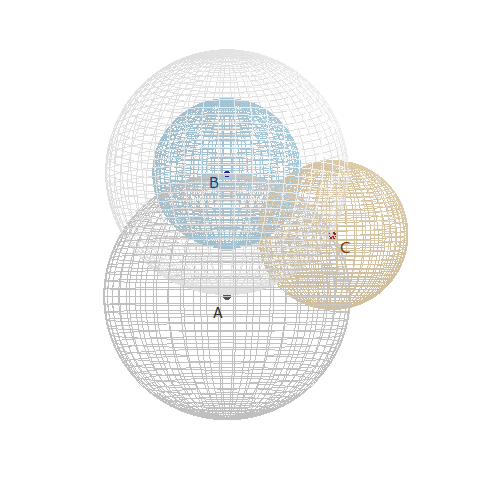
\includegraphics[width=10cm]{esferas.png}
     \end{center}  
     
    Todo esto asegura que el contraejemplo encontrado es válido.
    
\section{Asignación de trabajos}
Tenemos dos conjuntos, uno con $n$ trabajadores y otro con $n$ trabajos, y queremos asignar a cada trabajador un trabajo de forma
que el coste de realizar todos los trabajos sea mínimo. Dichos costes estarán proporcionados en una matriz cuadrada
de orden $n$. Queremos que cada trabajador realice únicamente un trabajo, y que no haya ningún trabajo sin asignar. 

Para resolver este problema, hemos implementado tres algoritmos greedy que se explican a continuación. 
	\subsection{Algoritmos}
		\subsubsection{Asignación por trabajador}
		Recorreremos la matriz desde el primer trabajador al último, buscando para cada trabajador el trabajo con coste mínimo que no esté ya asignado a algún trabajador. Almacenaremos los pares trabajador-trabajo en un vector, que será el valor de retorno. 
		
		\begin{algorithm}[H]
			\begin{algorithmic}[1]
				\REQUIRE \ \\
					\texttt{m}, matriz de costes, y $n$ orden de la matriz\\
				\STATE{\texttt{Crea una Asignacion vacía}}
				\STATE{\texttt{Crea un vector trabajosUsados de tamaño $n$ y lo rellena a false}}
				\STATE{\texttt{Minimo = -1}}
				\STATE{\texttt{posTrabajo = 0}}
		        \FORALL{Trabajador (i)}
		          \FORALL{Trabajo (j)}
		            \IF{!trabajosUsados[j]}
		            	\IF{Minimo < 0 || m[i][j] < Minimo}
		            		\STATE{\texttt{posTrabajo = j}}
		            	\ENDIF
		            \ENDIF
		          \ENDFOR
		          \STATE{\texttt{ Asignacion.push(pair(i,posTrabajo))} }
		          \STATE{\texttt{trabajosUsados[posTrabajo = true]} }
		        \ENDFOR  	
		        
				\RETURN{\texttt{Asignacion}}
			\end{algorithmic}
		    \caption{Asignación de trabajos}
		    \label{Asignación Trabajos}
		\end{algorithm}
		
	
		\subsubsection{Asignación por trabajo}
		En este caso, recorreremos la matriz por trabajos, buscando el trabajador que haga mínimo el coste de dicho trabajo y que no esté asignado a ninguno. De nuevo, devolveremos las asignaciones trabajador-trabajo en un vector. 
		
		Esta solución es simétrica a la anterior, con la única diferencia que recorre la matriz  primero por columnas 
		y después por filas, siendo antes al contrario. El código difiere únicamente en ese matiz. 
		
		\subsubsection{Búsqueda de mínimos globales}
		En este algoritmo, buscaremos el par trabajador-trabajo con coste mínimo en toda la matriz, siempre que los dos estén 
		libres. De esta forma obtendremos un mínimo global. Nuevamente, el valor de retorno será un vector con las asociaciones
		trabajador-trabajo. 
		
		\begin{algorithm}[H]
			\begin{algorithmic}[1]
				\REQUIRE \ \\
					\texttt{m}, matriz de costes, y $n$ orden de la matriz\\
				\STATE{\texttt{Crea una Asignacion vacía}}
				\STATE{\texttt{Crea dos vectores: trabajosUsados y trabajadoresUsados, de tamaño $n$ y los rellena a false}}
				\STATE{\texttt{Minimo = -1}}
				\STATE{\texttt{posTrabajo = 0\\ posTrabajador = 0}}
			       \FORALL{Fila}
			         \FORALL{Trabajador (j)}
			           \IF{!trabajadoresUsados[j]}
			           	 \FORALL{Trabajo (k)}
			               \IF{!trabajosUsados[j]}
			           	  	 \IF{Minimo < 0 || m[j][k] < Minimo}
			           			\STATE{\texttt{posTrabajo = k \\ posTrabajador = j}}
			           	     \ENDIF
			           	   \ENDIF
			             \ENDFOR
			           \ENDIF
			         \ENDFOR
			       \STATE{\texttt{Asignacion.push(pair(posTrabajador,posTrabajo))}}
			       \STATE{\texttt{trabajosUsados[posTrabajo] = true \\ trabajadoresUsados[posTrabajador] = true}}
			       \ENDFOR  	
				        
				\RETURN{\texttt{Asignacion}}
			\end{algorithmic}
			   \caption{Asignación de trabajos}
			   \label{Asignación Global}
		\end{algorithm}
		
	\subsection{Contraejemplos}
	Podemos encontrar contraejemplos muy sencillos para todos los algoritmos. Si consideramos la matriz de costes:
	
	\centering
	M = $\begin{pmatrix}
	    		1 & 2\\
	    		2 & 9\\
	\end{pmatrix}$
	\flushleft
	
	Los algoritmos por trabajos, por trabajadores y por mínimos globales asignarán: 
	\begin{itemize}
	\item{Trabajador 1 - Trabajo 1}
	\item{Trabajador 2 - Trabajo 2}
	\end{itemize}
		
	Solución con un coste de 10. Sin embargo, la solución 
		
	\begin{itemize}
	\item{Trabajador 1 - Trabajo 2}
	\item{Trabajador 2 - Trabajo 1}
	\end{itemize}
	  
	Tiene un coste de 4. Vemos de esta forma que estos algoritmos no proporcionan una solución óptima. 
	

\section{Asignación de aulas}
Tenemos los tiempos de comienzo y finalización de una serie de clases
($s_i$ y $f_i$, con $i\in\{1\ldots n\}$) y queremos encontrar el mínimo número de aulas necesarias
para dar esas $n$ clases.
Observamos que el problema es equivalente a uno de coloreo de grafos, para
el grafo no dirigido con función de adyacencia dada por:
$$\delta_{i,j}=\left\{\begin{array}{ll}
  true  & [s_i,f_i] \cap [s_j,f_j] \neq \emptyset \\
  false  & [s_i,f_i]\cap[s_j,f_j] = \emptyset\quad o\quad i=j\\
  \end{array}\right.$$

Es decir, habrá arista entre la clase $i-$ésima y la $j-$ésima si la
clase $i-$ésima y la $j-$ésima no pueden impartirse en el mismo aula.
  \subsection{Algoritmo}
\begin{algorithm}[H]
	\begin{algorithmic}[1]
		\REQUIRE \ \\
        	\texttt{clases}, array de $n$ objetos Clase, que almacena
				 un tiempo de inicialización y otro de 
				 finalización\\
     	\STATE{\texttt{adyadcentes}=$(\delta_{i,j})_{nxn}, i,j\in \{0\ldots \#clases - 1\}$}
     	\STATE{\texttt{sin\_colorear}= $\{0\ldots\#clases-1\}$}
     	\STATE{\texttt{color}=$[]$}
     	\STATE{\texttt{indice}=0}
	  \WHILE{\texttt{sin\_colorear}$\neq \emptyset$}
	    \STATE{\texttt{color[indice]=[sin\_colorear.pop\_front]}}
	    \FORALL{\texttt{v}$\in$\texttt{sin\_colorear}}
	      \IF{\textbf{no} \texttt{adyacentes[color[indice][0]][v]}}
		\STATE{\texttt{color[indice].push(v)}}
		\STATE{\texttt{sin\_colorear.delete(v)}}
	      \ENDIF
	    \ENDFOR
	    
	  \ENDWHILE
		\RETURN{$\#$\texttt{color}}
	\end{algorithmic}
    \caption{Asignación de aulas}
    \label{aulas}
\end{algorithm}


\subsection{Contraejemplo}
La existencia de grafos que no se pueden colorear mediante el algoritmo greedy, asegura que también existe una relación de clases para
las que la heurística presentada no proporciona la solución óptima. De hecho, hay casos, como el que se presenta a cotinuación,
en que el número de colores necesarios para colorear el grafo dependerá del orden de recorrido de sus nodos (esto se traduce en
el problema de la asignación de aulas en un distinto orden en el input de las clases):

     \begin{center}
	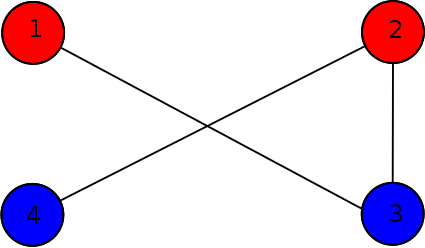
\includegraphics[width=5cm]{ej51.png}
	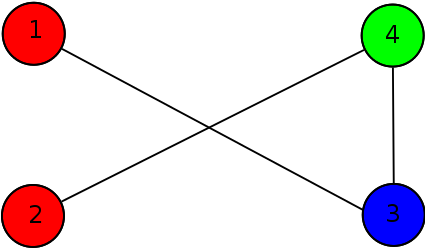
\includegraphics[width=5cm]{ej52.png}
     \end{center}  
     
\section{Memorias caché}
\label{cache}
%Heurística "Farthest-In-Future" en: https://www.cs.princeton.edu/courses/archive/spring13/cos423/lectures/04GreedyAlgorithmsI-2x2.pdf:
El problema de las memorias caché consiste en averiguar qué datos conviene eliminar en una caché, conociendo de antemano los datos que se van a pedir, para evitar lo máximo posible los fallos de caché.
  \subsection{Algoritmo}
La estrategia utilizada es reemplazar siempre el elemento que más tarde se vaya a utilizar (\textit{Farthest-in-future}) cada vez que se produzca un fallo de caché. Los primeros datos que se incluyen en caché son los primeros $k$ datos (sin considerar repeticiones) de la lista de peticiones.

Asumiremos en el algoritmo que tenemos implementadas una función \texttt{eliminaRepetidos}, que devuelve un array con una única ocurrencia de cada elemento del array pasado como argumento.

\begin{algorithm}[H]
	\begin{algorithmic}[1]
		\REQUIRE \ \\
        	\texttt{p}, array de $n$ peticiones\\
        	\texttt{k}, tamaño de la caché\\ \
     	\STATE{\texttt{fallos} = 0}\\
     	\STATE{\texttt{cache} = eliminaRepetidos(\texttt{p}).\texttt{slice}(0, k-1)}
	  \FORALL{\texttt{petición} $\in$ \texttt{p}}
	   \IF{\texttt{petición $\notin$ cache}}
		\STATE{\texttt{a\_eliminar} = Elemento de \texttt{p} en \texttt{cache} que más tardará en volver a ser necesitado}
		\STATE{\texttt{cache[cache.find(a\_eliminar)]} = \texttt{peticion}}
		\STATE{\texttt{fallos++}}
	   \ENDIF
	  \ENDFOR
	  
	  \RETURN{fallos}

	\end{algorithmic}
    \caption{Optimización de memoria caché}
    \label{memory}
\end{algorithm}

 El mayor inconveniente de esta heurística frente a las clásicas heurísticas FIFO(First In, First Out), LIFO(Last In, First Out), LRU(Least Recently Used) y LFU(Least Frequently Used) para asignación de memoria caché es que, dado que necesita conocer con anterioridad las peticiones que se le harán, no se puede implementar en un sistema de tiempo real.
 
  \subsection{Teorema de Bélády}
  Veamos que este algoritmo es óptimo.
  Primero, tenemos que definir lo que es una tabla de expulsiones/inserciones reducida.
  
  \begin{mydef}
    Una tabla de expulsiones/inserciones reducida es aquella que sólo inserta un elemento en caché cuando dicho elemento es requerido.
  \end{mydef}
  
  \begin{theorem}[Teorema de Bélády]
    Farthest-in-future es el algoritmo de expulsiones óptimo.
  \end{theorem}

  \begin{proof}[\textbf{Demostración:}]
  	Previamente, vamos a probar un lema.
  
	  \begin{proof}[\textbf{Lema:}]
	    \textit{
	      Dada una tabla de expulsiones/inserciones no reducida $S$, se puede transformar en una reducida $S'$ sin añadir ninguna expulsión  
	    }
	    
	    Lo probaremos por inducción sobre el número de elementos que no se insertan cuando se piden.
	    
	    Supongamos que $S$ inserta en la caché un elemento $d$ en un instante $t$(antes de ser requerido), y $c$
	    es el elemento que $S$ saca.
	    
	    Pueden darse dos casos:
	    \begin{itemize}
	      \item \textbf{Caso 1: } $d$ es expulsado antes de su próxima petición.\\
	      En este caso, anulamos la inserción de $d$ y la expulsión de $c$.
	      \item \textbf{Caso 2: } $d$ es requerido antes de ser expulsado. \\
	      En este caso, retrasamos la inserción de $d$ y la expulsión de $c$.
	    \end{itemize}
	    
	    Y lo que nos queda, es la tabla de expulsiones/inserciones reducida $S'$.
	    %Completo
	  \end{proof}

	%Incompleto
  \end{proof}
  
  
\section{Implementaciones}
   \subsection{Terminales de venta}
      Implementamos el algoritmo diseñado en Ruby.
  
      \small
	\texttt{% Generator: GNU source-highlight, by Lorenzo Bettini, http://www.gnu.org/software/src-highlite
\noindent
\mbox{}\textbf{\textcolor{Blue}{def}}\ cambio\ \textcolor{BrickRed}{(}monedas\textcolor{BrickRed}{,}\ precio\textcolor{BrickRed}{)} \\
\mbox{}\ \ vuelta\ \textcolor{BrickRed}{=}\ \textcolor{BrickRed}{[]} \\
\mbox{} \\
\mbox{}\ \ monedas\textcolor{BrickRed}{.}sort\textcolor{BrickRed}{.}reverse\textcolor{BrickRed}{.}each\ \textcolor{Red}{\{}\ \textcolor{BrickRed}{$|$}moneda\textcolor{BrickRed}{$|$} \\
\mbox{}\ \ \ \ numero$\_$monedas\ \textcolor{BrickRed}{=}\ precio\ \textcolor{BrickRed}{/}\ moneda \\
\mbox{}\ \ \ \ precio\ \textcolor{BrickRed}{=}\ precio\ \textcolor{BrickRed}{-}\ numero$\_$monedas\textcolor{BrickRed}{*}moneda \\
\mbox{} \\
\mbox{}\ \ \ \ vuelta\textcolor{BrickRed}{.}push\ \textcolor{BrickRed}{[}moneda\textcolor{BrickRed}{,}\ numero$\_$monedas\textcolor{BrickRed}{]} \\
\mbox{}\ \ \textcolor{Red}{\}} \\
\mbox{} \\
\mbox{}\ \ \textbf{\textcolor{Blue}{return}}\ vuelta \\
\mbox{}\textbf{\textcolor{Blue}{end}} \\
\mbox{}
}
      \normalsize
   
   \subsection{Red de comunicaciones}
      Implementamos la construcción de grafos euclídeos a partir del conjunto de puntos, así como el algoritmo de Kruskal y
      el dibujado del grafo euclídeo.
      
      \small
	\texttt{% Generator: GNU source-highlight, by Lorenzo Bettini, http://www.gnu.org/software/src-highlite
\noindent
\mbox{}\textit{\textcolor{Brown}{\#!/usr/bin/env\ python}} \\
\mbox{}\textit{\textcolor{Brown}{\#\ encoding:\ utf-8}} \\
\mbox{} \\
\mbox{}\textit{\textcolor{Brown}{\#\ Siguiendo\ el\ ejemplo\ de\ https://github.com/israelst/Algorithms-Book-\/-Python/blob/master/5-Greedy-algorithms/kruskal.py}} \\
\mbox{}\textbf{\textcolor{RoyalBlue}{from}}\ sets\ \textbf{\textcolor{RoyalBlue}{import}}\ Set \\
\mbox{} \\
\mbox{}\textit{\textcolor{Brown}{\#\ Formato\ de\ los\ grafos.}} \\
\mbox{}empty$\_$graph\ \textcolor{BrickRed}{=}\ \textcolor{BrickRed}{\{} \\
\mbox{}\ \ \ \ \texttt{\textcolor{Red}{'vertices'}}\textcolor{BrickRed}{:}\ \textcolor{BrickRed}{[],} \\
\mbox{}\ \ \ \ \texttt{\textcolor{Red}{'edges'}}\textcolor{BrickRed}{:}\ \textbf{\textcolor{Black}{set}}\textcolor{BrickRed}{()} \\
\mbox{}\textcolor{BrickRed}{\}} \\
\mbox{} \\
\mbox{}\textbf{\textcolor{Blue}{def}}\ \textbf{\textcolor{Black}{euclideanGraph}}\textcolor{BrickRed}{(}points\textcolor{BrickRed}{):} \\
\mbox{}\ \ \ \ graph\ \textcolor{BrickRed}{=}\ \textcolor{BrickRed}{\{} \\
\mbox{}\ \ \ \ \ \ \ \ \texttt{\textcolor{Red}{'vertices'}}\textcolor{BrickRed}{:}\ \textcolor{BrickRed}{[],} \\
\mbox{}\ \ \ \ \ \ \ \ \texttt{\textcolor{Red}{'edges'}}\textcolor{BrickRed}{:}\ \textbf{\textcolor{Black}{set}}\textcolor{BrickRed}{()} \\
\mbox{}\ \ \ \ \textcolor{BrickRed}{\}} \\
\mbox{} \\
\mbox{}\ \ \ \ \textit{\textcolor{Brown}{\#\ Añade\ los\ nodos.}} \\
\mbox{}\ \ \ \ \textbf{\textcolor{Blue}{for}}\ p\ \textbf{\textcolor{Blue}{in}}\ points\textcolor{BrickRed}{:} \\
\mbox{}\ \ \ \ \ \ \ \ graph\textcolor{BrickRed}{[}\texttt{\textcolor{Red}{'vertices'}}\textcolor{BrickRed}{].}\textbf{\textcolor{Black}{append}}\textcolor{BrickRed}{(}p\textcolor{BrickRed}{)} \\
\mbox{}\ \ \ \  \\
\mbox{}\ \ \ \ \textit{\textcolor{Brown}{\#\ Añade\ una\ arista\ de\ peso\ distancia\ entre\ cada\ dos\ puntos.}} \\
\mbox{}\ \ \ \ \textbf{\textcolor{Blue}{for}}\ i\ \textbf{\textcolor{Blue}{in}}\ \textbf{\textcolor{Black}{range}}\textcolor{BrickRed}{(}\textbf{\textcolor{Black}{len}}\textcolor{BrickRed}{(}points\textcolor{BrickRed}{)):}\  \\
\mbox{}\ \ \ \ \ \ \ \ \textbf{\textcolor{Blue}{for}}\ j\ \textbf{\textcolor{Blue}{in}}\ \textbf{\textcolor{Black}{range}}\textcolor{BrickRed}{(}i\textcolor{BrickRed}{+}\textcolor{Purple}{1}\textcolor{BrickRed}{,}\textbf{\textcolor{Black}{len}}\textcolor{BrickRed}{(}points\textcolor{BrickRed}{)):} \\
\mbox{}\ \ \ \ \ \ \ \ \ \ \ \ p\textcolor{BrickRed}{,}q\ \textcolor{BrickRed}{=}\ points\textcolor{BrickRed}{[}i\textcolor{BrickRed}{],}points\textcolor{BrickRed}{[}j\textcolor{BrickRed}{]} \\
\mbox{}\ \ \ \ \ \ \ \ \ \ \ \ edge\ \textcolor{BrickRed}{=}\ \textcolor{BrickRed}{(}p\textcolor{BrickRed}{,}q\textcolor{BrickRed}{,}\textbf{\textcolor{Black}{dist}}\textcolor{BrickRed}{(}p\textcolor{BrickRed}{,}q\textcolor{BrickRed}{))} \\
\mbox{}\ \ \ \ \ \ \ \ \ \ \ \ graph\textcolor{BrickRed}{[}\texttt{\textcolor{Red}{'edges'}}\textcolor{BrickRed}{].}\textbf{\textcolor{Black}{add}}\textcolor{BrickRed}{(}edge\textcolor{BrickRed}{)} \\
\mbox{}\ \ \ \ \ \ \ \ \ \ \ \  \\
\mbox{}\ \ \ \ \textbf{\textcolor{Blue}{return}}\ graph \\
\mbox{} \\
\mbox{} \\
\mbox{}\textbf{\textcolor{RoyalBlue}{from}}\ math\ \textbf{\textcolor{RoyalBlue}{import}}\ sqrt \\
\mbox{}\textbf{\textcolor{Blue}{def}}\ \textbf{\textcolor{Black}{dist}}\textcolor{BrickRed}{(}p\textcolor{BrickRed}{,}q\textcolor{BrickRed}{):} \\
\mbox{}\textit{\textcolor{Brown}{\ \ \ \ "{}"{}"{}\ Devuelve\ distancia\ euclídea\ entre\ dos\ puntos."{}"{}"{}}} \\
\mbox{}\ \ \ \ p\textcolor{BrickRed}{,}q\ \textcolor{BrickRed}{=}\ \textbf{\textcolor{Black}{list}}\textcolor{BrickRed}{(}p\textcolor{BrickRed}{),}\textbf{\textcolor{Black}{list}}\textcolor{BrickRed}{(}q\textcolor{BrickRed}{)} \\
\mbox{}\ \ \ \ sum\ \textcolor{BrickRed}{=}\ \textcolor{Purple}{0} \\
\mbox{}\ \ \ \ \textbf{\textcolor{Blue}{for}}\ i\ \textbf{\textcolor{Blue}{in}}\ \textbf{\textcolor{Black}{range}}\textcolor{BrickRed}{(}\textbf{\textcolor{Black}{min}}\textcolor{BrickRed}{(}\textbf{\textcolor{Black}{len}}\textcolor{BrickRed}{(}p\textcolor{BrickRed}{),}\textbf{\textcolor{Black}{len}}\textcolor{BrickRed}{(}q\textcolor{BrickRed}{))):} \\
\mbox{}\ \ \ \ \ \ \ \ sum\ \textcolor{BrickRed}{=}\ sum\ \textcolor{BrickRed}{+}\ \textcolor{BrickRed}{(}p\textcolor{BrickRed}{[}i\textcolor{BrickRed}{]-}q\textcolor{BrickRed}{[}i\textcolor{BrickRed}{])**}\textcolor{Purple}{2} \\
\mbox{}\ \ \ \ \textbf{\textcolor{Blue}{return}}\ \textbf{\textcolor{Black}{sqrt}}\textcolor{BrickRed}{(}sum\textcolor{BrickRed}{)} \\
\mbox{} \\
\mbox{} \\
\mbox{}\textit{\textcolor{Brown}{\#\ Dibujando\ grafos\ euclídeos.}} \\
\mbox{}\textbf{\textcolor{RoyalBlue}{from}}\ pylab\ \textbf{\textcolor{RoyalBlue}{import}}\ plot\textcolor{BrickRed}{,}\ show \\
\mbox{}\textbf{\textcolor{Blue}{def}}\ \textbf{\textcolor{Black}{plotGraph}}\textcolor{BrickRed}{(}graph\textcolor{BrickRed}{,}\ clr\textcolor{BrickRed}{=}\texttt{\textcolor{Red}{'k'}}\textcolor{BrickRed}{):} \\
\mbox{}\ \ \ \ \textit{\textcolor{Brown}{\#\ Dibuja\ líneas}} \\
\mbox{}\ \ \ \ \textbf{\textcolor{Blue}{for}}\ edge\ \textbf{\textcolor{Blue}{in}}\ graph\textcolor{BrickRed}{[}\texttt{\textcolor{Red}{'edges'}}\textcolor{BrickRed}{]:} \\
\mbox{}\ \ \ \ \ \ \ \ p\textcolor{BrickRed}{,}q\textcolor{BrickRed}{,}weight\ \textcolor{BrickRed}{=}\ edge \\
\mbox{}\ \ \ \ \ \ \ \ x1\textcolor{BrickRed}{,}y1\ \textcolor{BrickRed}{=}\ p \\
\mbox{}\ \ \ \ \ \ \ \ x2\textcolor{BrickRed}{,}y2\ \textcolor{BrickRed}{=}\ q \\
\mbox{}\ \ \ \ \ \ \ \ \textbf{\textcolor{Black}{plot}}\textcolor{BrickRed}{([}x1\textcolor{BrickRed}{,}x2\textcolor{BrickRed}{],[}y1\textcolor{BrickRed}{,}y2\textcolor{BrickRed}{],}linestyle\textcolor{BrickRed}{=}\texttt{\textcolor{Red}{'-'}}\textcolor{BrickRed}{,}linewidth\textcolor{BrickRed}{=}\textcolor{Purple}{3}\textcolor{BrickRed}{,}\ color\textcolor{BrickRed}{=}clr\textcolor{BrickRed}{)} \\
\mbox{} \\
\mbox{}\ \ \ \ \textit{\textcolor{Brown}{\#\ Dibuja\ puntos}} \\
\mbox{}\ \ \ \ \textbf{\textcolor{Blue}{for}}\ point\ \textbf{\textcolor{Blue}{in}}\ graph\textcolor{BrickRed}{[}\texttt{\textcolor{Red}{'vertices'}}\textcolor{BrickRed}{]:} \\
\mbox{}\ \ \ \ \ \ \ \ x\textcolor{BrickRed}{,}y\ \textcolor{BrickRed}{=}\ point \\
\mbox{}\ \ \ \ \ \ \ \ \textbf{\textcolor{Black}{plot}}\textcolor{BrickRed}{(}x\textcolor{BrickRed}{,}y\textcolor{BrickRed}{,}\texttt{\textcolor{Red}{'ro'}}\textcolor{BrickRed}{,}markersize\textcolor{BrickRed}{=}\textcolor{Purple}{15}\textcolor{BrickRed}{)} \\
\mbox{} \\
\mbox{} \\
\mbox{}\textbf{\textcolor{Blue}{def}}\ \textbf{\textcolor{Black}{kruskal}}\textcolor{BrickRed}{(}graph\textcolor{BrickRed}{,}\ limit\textcolor{BrickRed}{=}\textcolor{Purple}{0}\textcolor{BrickRed}{):} \\
\mbox{}\ \ \ \ \textit{\textcolor{Brown}{\#\ Árbol\ generador\ minimal.}} \\
\mbox{}\ \ \ \ minimum$\_$spanning$\_$tree\ \textcolor{BrickRed}{=}\ \textbf{\textcolor{Black}{set}}\textcolor{BrickRed}{()} \\
\mbox{} \\
\mbox{}\ \ \ \ \textit{\textcolor{Brown}{\#\ Define\ una\ componente\ conexa\ para\ cada\ vértice.}} \\
\mbox{}\ \ \ \ components\ \textcolor{BrickRed}{=}\ \textbf{\textcolor{Black}{dict}}\textcolor{BrickRed}{()} \\
\mbox{}\ \ \ \ \textbf{\textcolor{Blue}{for}}\ v\ \textbf{\textcolor{Blue}{in}}\ graph\textcolor{BrickRed}{[}\texttt{\textcolor{Red}{'vertices'}}\textcolor{BrickRed}{]:} \\
\mbox{}\ \ \ \ \ \ \ \ components\textcolor{BrickRed}{[}v\textcolor{BrickRed}{]}\ \textcolor{BrickRed}{=}\ \textbf{\textcolor{Black}{Set}}\textcolor{BrickRed}{([}v\textcolor{BrickRed}{])} \\
\mbox{}\ \ \ \  \\
\mbox{}\ \ \ \ \textit{\textcolor{Brown}{\#\ Toma\ el\ mínimo\ de\ la\ lista\ de\ aristas.}} \\
\mbox{}\ \ \ \ edgesList\ \textcolor{BrickRed}{=}\ \textbf{\textcolor{Black}{list}}\textcolor{BrickRed}{(}graph\textcolor{BrickRed}{[}\texttt{\textcolor{Red}{'edges'}}\textcolor{BrickRed}{])} \\
\mbox{}\ \ \ \ edgesList\textcolor{BrickRed}{.}\textbf{\textcolor{Black}{sort}}\textcolor{BrickRed}{(}key\textcolor{BrickRed}{=}\textbf{\textcolor{Blue}{lambda}}\ edge\textcolor{BrickRed}{:}edge\textcolor{BrickRed}{[}\textcolor{Purple}{2}\textcolor{BrickRed}{])} \\
\mbox{} \\
\mbox{}\ \ \ \ \textit{\textcolor{Brown}{\#\ Considera\ cada\ arista\ del\ vértice.}} \\
\mbox{}\ \ \ \ \textbf{\textcolor{Blue}{for}}\ edge\ \textbf{\textcolor{Blue}{in}}\ edgesList\textcolor{BrickRed}{:} \\
\mbox{}\ \ \ \ \ \ \ \ node1\textcolor{BrickRed}{,}\ node2\textcolor{BrickRed}{,}\ weight\ \textcolor{BrickRed}{=}\ edge \\
\mbox{}\ \ \ \ \ \ \ \ \textbf{\textcolor{Blue}{if}}\ components\textcolor{BrickRed}{[}node1\textcolor{BrickRed}{]}\ \textcolor{BrickRed}{!=}\ components\textcolor{BrickRed}{[}node2\textcolor{BrickRed}{]}\ \textbf{\textcolor{Blue}{and}}\ \textbf{\textcolor{Black}{len}}\textcolor{BrickRed}{(}minimum$\_$spanning$\_$tree\textcolor{BrickRed}{)}\ \textcolor{BrickRed}{\textless{}}\ \textbf{\textcolor{Black}{len}}\textcolor{BrickRed}{(}graph\textcolor{BrickRed}{[}\texttt{\textcolor{Red}{'vertices'}}\textcolor{BrickRed}{])-}limit\textcolor{BrickRed}{:} \\
\mbox{}\ \ \ \ \ \ \ \ \ \ \ \ \textit{\textcolor{Brown}{\#\ Realiza\ la\ unión\ de\ las\ componentes.}} \\
\mbox{}\ \ \ \ \ \ \ \ \ \ \ \ \textit{\textcolor{Brown}{\#\ Los\ nodos\ del\ segundo\ componente\ pasan\ al\ primero.}} \\
\mbox{}\ \ \ \ \ \ \ \ \ \ \ \ \textbf{\textcolor{Blue}{for}}\ node\ \textbf{\textcolor{Blue}{in}}\ components\textcolor{BrickRed}{[}node2\textcolor{BrickRed}{]:} \\
\mbox{}\ \ \ \ \ \ \ \ \ \ \ \ \ \ \ \ components\textcolor{BrickRed}{[}node\textcolor{BrickRed}{]}\ \textcolor{BrickRed}{=}\ components\textcolor{BrickRed}{[}node1\textcolor{BrickRed}{]} \\
\mbox{}\ \ \ \ \ \ \ \ \ \ \ \ \ \ \ \ components\textcolor{BrickRed}{[}node1\textcolor{BrickRed}{].}\textbf{\textcolor{Black}{add}}\textcolor{BrickRed}{(}node\textcolor{BrickRed}{)} \\
\mbox{}\ \ \ \ \ \ \ \ \ \ \ \  \\
\mbox{}\ \ \ \ \ \ \ \ \ \ \ \ \textit{\textcolor{Brown}{\#\ Añade\ la\ arista\ al\ árbol\ generador.}} \\
\mbox{}\ \ \ \ \ \ \ \ \ \ \ \ minimum$\_$spanning$\_$tree\textcolor{BrickRed}{.}\textbf{\textcolor{Black}{add}}\textcolor{BrickRed}{((}node1\textcolor{BrickRed}{,}\ node2\textcolor{BrickRed}{,}\ weight\textcolor{BrickRed}{))} \\
\mbox{} \\
\mbox{}\ \ \ \ \textit{\textcolor{Brown}{\#\ Genera\ el\ grafo\ pedido}} \\
\mbox{}\ \ \ \ mstree\ \textcolor{BrickRed}{=}\ \textcolor{BrickRed}{\{} \\
\mbox{}\ \ \ \ \ \ \ \ \texttt{\textcolor{Red}{'vertices'}}\textcolor{BrickRed}{:}\ graph\textcolor{BrickRed}{[}\texttt{\textcolor{Red}{'vertices'}}\textcolor{BrickRed}{],} \\
\mbox{}\ \ \ \ \ \ \ \ \texttt{\textcolor{Red}{'edges'}}\textcolor{BrickRed}{:}\ minimum$\_$spanning$\_$tree \\
\mbox{}\ \ \ \ \textcolor{BrickRed}{\}} \\
\mbox{} \\
\mbox{}\ \ \ \ \textbf{\textcolor{Blue}{return}}\ mstree \\
\mbox{} \\
\mbox{} \\
\mbox{}\textbf{\textcolor{Blue}{def}}\ \textbf{\textcolor{Black}{readPoints}}\textcolor{BrickRed}{():} \\
\mbox{}\textit{\textcolor{Brown}{\ \ \ \ "{}"{}"{}}} \\
\mbox{}\textit{\textcolor{Brown}{\ \ \ \ Lee\ puntos\ con\ el\ formato\ de\ entrada\ siguiente:}} \\
\mbox{}\textit{\textcolor{Brown}{\ \ \ \ \ \ n}} \\
\mbox{}\textit{\textcolor{Brown}{\ \ \ \ \ \ x\ y}} \\
\mbox{}\textit{\textcolor{Brown}{\ \ \ \ \ \ x\ y}} \\
\mbox{}\textit{\textcolor{Brown}{\ \ \ \ \ \ x\ y}} \\
\mbox{}\textit{\textcolor{Brown}{\ \ \ \ \ \ (...)}} \\
\mbox{}\textit{\textcolor{Brown}{\ \ \ \ donde\ n\ es\ el\ número\ de\ puntos\ y\ [x,y]\ son\ las\ coordenadas\ de\ un\ punto.}} \\
\mbox{}\textit{\textcolor{Brown}{\ \ \ \ "{}"{}"{}}} \\
\mbox{}\ \ \ \ points\ \textcolor{BrickRed}{=}\ \textcolor{BrickRed}{[]} \\
\mbox{} \\
\mbox{}\ \ \ \ \textbf{\textcolor{Blue}{for}}\ i\ \textbf{\textcolor{Blue}{in}}\ \textbf{\textcolor{Black}{range}}\textcolor{BrickRed}{(}\textbf{\textcolor{Black}{int}}\textcolor{BrickRed}{(}\textbf{\textcolor{Black}{input}}\textcolor{BrickRed}{())):} \\
\mbox{}\ \ \ \ \ \ \ \ x\textcolor{BrickRed}{,}y\ \textcolor{BrickRed}{=}\ \textbf{\textcolor{Black}{raw$\_$input}}\textcolor{BrickRed}{().}\textbf{\textcolor{Black}{strip}}\textcolor{BrickRed}{().}\textbf{\textcolor{Black}{split}}\textcolor{BrickRed}{()} \\
\mbox{}\ \ \ \ \ \ \ \ x\textcolor{BrickRed}{,}y\ \textcolor{BrickRed}{=}\ \textbf{\textcolor{Black}{int}}\textcolor{BrickRed}{(}x\textcolor{BrickRed}{),}\ \textbf{\textcolor{Black}{int}}\textcolor{BrickRed}{(}y\textcolor{BrickRed}{)} \\
\mbox{}\ \ \ \ \ \ \ \ points\textcolor{BrickRed}{.}\textbf{\textcolor{Black}{append}}\textcolor{BrickRed}{((}x\textcolor{BrickRed}{,}y\textcolor{BrickRed}{))} \\
\mbox{} \\
\mbox{}\ \ \ \ \textbf{\textcolor{Blue}{return}}\ points \\
\mbox{} \\
\mbox{} \\
\mbox{}\textbf{\textcolor{Blue}{if}}\ $\_$$\_$name$\_$$\_$\ \textcolor{BrickRed}{==}\ \texttt{\textcolor{Red}{"{}$\_$$\_$main$\_$$\_$"{}}}\textcolor{BrickRed}{:} \\
\mbox{}\ \ \ \ points\ \textcolor{BrickRed}{=}\ \textbf{\textcolor{Black}{readPoints}}\textcolor{BrickRed}{()} \\
\mbox{}\ \ \ \ graph\ \textcolor{BrickRed}{=}\ \textbf{\textcolor{Black}{euclideanGraph}}\textcolor{BrickRed}{(}points\textcolor{BrickRed}{)} \\
\mbox{}\ \ \ \ solution\ \textcolor{BrickRed}{=}\ \textbf{\textcolor{Black}{kruskal}}\textcolor{BrickRed}{(}graph\textcolor{BrickRed}{)} \\
\mbox{}\ \ \ \  \\
\mbox{}\ \ \ \ \textit{\textcolor{Brown}{\#plotGraph(graph,'k')}} \\
\mbox{}\ \ \ \ \textbf{\textcolor{Black}{plotGraph}}\textcolor{BrickRed}{(}solution\textcolor{BrickRed}{,}\texttt{\textcolor{Red}{'k'}}\textcolor{BrickRed}{)} \\
\mbox{}\ \ \ \ \textbf{\textcolor{Black}{show}}\textcolor{BrickRed}{()} \\
\mbox{}
}
      \normalsize
    
   \subsection{Segmentación de clientes}
      Se incluye a continuación una implementación en Python, utilizando como base la implementación del ejercicio anterior.\\
        \small
	\texttt{% Generator: GNU source-highlight, by Lorenzo Bettini, http://www.gnu.org/software/src-highlite
\noindent
\mbox{}\textbf{\textcolor{RoyalBlue}{import}}\ euclidean$\_$graph\ as\ eg \\
\mbox{}\textbf{\textcolor{RoyalBlue}{import}}\ sys \\
\mbox{} \\
\mbox{}\textbf{\textcolor{Blue}{def}}\ \textbf{\textcolor{Black}{readKPoints}}\textcolor{BrickRed}{():} \\
\mbox{}\textit{\textcolor{Brown}{\ \ \ \ "{}"{}"{}}} \\
\mbox{}\textit{\textcolor{Brown}{\ \ \ \ Lee\ puntos\ con\ el\ formato\ de\ entrada\ siguiente:}} \\
\mbox{}\textit{\textcolor{Brown}{\ \ \ \ \ \ n}} \\
\mbox{}\textit{\textcolor{Brown}{\ \ \ \ \ \ x1\ x2\ x3\ ..\ xk}} \\
\mbox{}\textit{\textcolor{Brown}{\ \ \ \ \ \ y1\ y2\ y3\ ..\ yk}} \\
\mbox{}\textit{\textcolor{Brown}{\ \ \ \ \ \ z1\ z2\ z3\ ..\ zk}} \\
\mbox{}\textit{\textcolor{Brown}{\ \ \ \ \ \ (...)}} \\
\mbox{}\textit{\textcolor{Brown}{\ \ \ \ donde\ n\ es\ el\ número\ de\ puntos,\ d\ es\ la\ dimensión\ y\ [x1,x2,x3...xk]\ }} \\
\mbox{}\textit{\textcolor{Brown}{\ \ \ \ son\ las\ coordenadas\ de\ un\ punto.}} \\
\mbox{}\textit{\textcolor{Brown}{\ \ \ \ "{}"{}"{}}} \\
\mbox{}\ \ \ \ points\ \textcolor{BrickRed}{=}\ \textcolor{BrickRed}{[]} \\
\mbox{}\ \ \ \ n\ \textcolor{BrickRed}{=}\ \textbf{\textcolor{Black}{int}}\textcolor{BrickRed}{(}\textbf{\textcolor{Black}{input}}\textcolor{BrickRed}{())} \\
\mbox{} \\
\mbox{}\ \ \ \ \textbf{\textcolor{Blue}{for}}\ i\ \textbf{\textcolor{Blue}{in}}\ \textbf{\textcolor{Black}{range}}\textcolor{BrickRed}{(}n\textcolor{BrickRed}{):} \\
\mbox{}\ \ \ \ \ \ \ \ p\ \textcolor{BrickRed}{=}\ \textbf{\textcolor{Black}{raw$\_$input}}\textcolor{BrickRed}{().}\textbf{\textcolor{Black}{strip}}\textcolor{BrickRed}{().}\textbf{\textcolor{Black}{split}}\textcolor{BrickRed}{()} \\
\mbox{}\ \ \ \ \ \ \ \ p\ \textcolor{BrickRed}{=}\ \textcolor{BrickRed}{[}\textbf{\textcolor{Black}{int}}\textcolor{BrickRed}{(}x\textcolor{BrickRed}{)}\ \textbf{\textcolor{Blue}{for}}\ x\ \textbf{\textcolor{Blue}{in}}\ p\textcolor{BrickRed}{]} \\
\mbox{}\ \ \ \ \ \ \ \ points\textcolor{BrickRed}{.}\textbf{\textcolor{Black}{append}}\textcolor{BrickRed}{(}\textbf{\textcolor{Black}{tuple}}\textcolor{BrickRed}{(}p\textcolor{BrickRed}{))} \\
\mbox{} \\
\mbox{}\ \ \ \ \textbf{\textcolor{Blue}{return}}\ points \\
\mbox{} \\
\mbox{}\textbf{\textcolor{Blue}{if}}\ $\_$$\_$name$\_$$\_$\ \textcolor{BrickRed}{==}\ \texttt{\textcolor{Red}{"{}$\_$$\_$main$\_$$\_$"{}}}\textcolor{BrickRed}{:} \\
\mbox{}\ \ \ \ points\ \textcolor{BrickRed}{=}\ \textbf{\textcolor{Black}{readKPoints}}\textcolor{BrickRed}{()} \\
\mbox{}\ \ \ \ graph\ \textcolor{BrickRed}{=}\ eg\textcolor{BrickRed}{.}\textbf{\textcolor{Black}{euclideanGraph}}\textcolor{BrickRed}{(}points\textcolor{BrickRed}{)} \\
\mbox{}\ \ \ \  \\
\mbox{}\ \ \ \ k\ \textcolor{BrickRed}{=}\ \textbf{\textcolor{Black}{int}}\textcolor{BrickRed}{(}sys\textcolor{BrickRed}{.}argv\textcolor{BrickRed}{[}\textcolor{Purple}{1}\textcolor{BrickRed}{])} \\
\mbox{}\ \ \ \ solution\ \textcolor{BrickRed}{=}\ eg\textcolor{BrickRed}{.}\textbf{\textcolor{Black}{kruskal}}\textcolor{BrickRed}{(}graph\textcolor{BrickRed}{,}k\textcolor{BrickRed}{)} \\
\mbox{} \\
\mbox{}\ \ \ \ eg\textcolor{BrickRed}{.}\textbf{\textcolor{Black}{plotGraph}}\textcolor{BrickRed}{(}solution\textcolor{BrickRed}{,}\texttt{\textcolor{Red}{'k'}}\textcolor{BrickRed}{)} \\
\mbox{}\ \ \ \ eg\textcolor{BrickRed}{.}\textbf{\textcolor{Black}{show}}\textcolor{BrickRed}{()} \\
\mbox{}\ \ \ \  \\
\mbox{}
}
	\normalsize
	
	\subsection{Asignación de trabajos}
	Implementamos el algoritmo en C++
	
	\small
	\texttt{% Generator: GNU source-highlight, by Lorenzo Bettini, http://www.gnu.org/software/src-highlite
\noindent
\mbox{}\textit{\textcolor{Brown}{//\ \ Problema\ 4:\ Asignación\ de\ trabajos.\ Utilizando\ heurística\ greedy.\ Se\ implementan\ 3\ heurísticas\ greedy.\ }} \\
\mbox{} \\
\mbox{}\textbf{\textcolor{RoyalBlue}{\#include}}\ \texttt{\textcolor{Red}{\textless{}iostream\textgreater{}}} \\
\mbox{}\textbf{\textcolor{RoyalBlue}{\#include}}\ \texttt{\textcolor{Red}{\textless{}vector\textgreater{}}} \\
\mbox{} \\
\mbox{}\textbf{\textcolor{Blue}{using}}\ \textbf{\textcolor{Blue}{namespace}}\ std\textcolor{BrickRed}{;} \\
\mbox{} \\
\mbox{}\textbf{\textcolor{Blue}{typedef}}\ \textcolor{TealBlue}{vector\textless{}pair\textless{}int,\ int\textgreater{}\ \textgreater{}}\ Asignacion\textcolor{BrickRed}{;} \\
\mbox{} \\
\mbox{}\textit{\textcolor{Brown}{/*\ }} \\
\mbox{}\textit{\textcolor{Brown}{\ \ \ \ Heurística\ greedyTrabajador.\ Recorre\ la\ matriz\ por\ trabajador\ (filas)\ y\ busca\ el\ trabajo\ que\ aun\ no\ esté\ asignado\ }} \\
\mbox{}\textit{\textcolor{Brown}{\ \ \ \ a\ ningún\ trabajado\ con\ coste\ mínimo,\ y\ lo\ asigna\ al\ trabajador\ actual.\ }} \\
\mbox{}\textit{\textcolor{Brown}{\ \ \ \ Tiene\ una\ eficiencia\ cuadrática,\ pues\ consta\ de\ dos\ bucles\ for\ anidados.}} \\
\mbox{}\textit{\textcolor{Brown}{*/}} \\
\mbox{}\textcolor{TealBlue}{Asignacion}\ \textbf{\textcolor{Black}{greedyTrabajador}}\textcolor{BrickRed}{(}\textcolor{ForestGreen}{double}\ \textcolor{BrickRed}{**}m\textcolor{BrickRed}{,}\ \textcolor{ForestGreen}{int}\ size\textcolor{BrickRed}{)}\textcolor{Red}{\{} \\
\mbox{}\ \ \ \  \\
\mbox{}\ \ \ \ \textcolor{TealBlue}{Asignacion}\ asignacion$\_$final\textcolor{BrickRed}{;}\  \\
\mbox{}\ \ \ \ \textcolor{ForestGreen}{bool}\ trabajos$\_$usados\textcolor{BrickRed}{[}size\textcolor{BrickRed}{];}\  \\
\mbox{}\ \ \ \ \textbf{\textcolor{Blue}{for}}\ \textcolor{BrickRed}{(}\textcolor{ForestGreen}{int}\ i\ \textcolor{BrickRed}{=}\ \textcolor{Purple}{0}\textcolor{BrickRed}{;}\ i\ \textcolor{BrickRed}{\textless{}}\ size\textcolor{BrickRed}{;}\ i\textcolor{BrickRed}{++)} \\
\mbox{}\ \ \ \ \ \ \ \ trabajos$\_$usados\textcolor{BrickRed}{[}i\textcolor{BrickRed}{]}\ \textcolor{BrickRed}{=}\ \textbf{\textcolor{Blue}{false}}\textcolor{BrickRed}{;}\  \\
\mbox{}\ \ \ \  \\
\mbox{}\ \ \ \ \textbf{\textcolor{Blue}{for}}\ \textcolor{BrickRed}{(}\textcolor{ForestGreen}{int}\ i\ \textcolor{BrickRed}{=}\ \textcolor{Purple}{0}\textcolor{BrickRed}{;}\ i\ \textcolor{BrickRed}{\textless{}}\ size\textcolor{BrickRed}{;}\ i\textcolor{BrickRed}{++)}\textcolor{Red}{\{}\ \ \ \ \ \ \ \ \ \ \ \ \ \ \ \ \textit{\textcolor{Brown}{//\ Recorremos\ los\ trabajadores.\ }} \\
\mbox{}\ \ \ \ \ \ \ \ \textcolor{ForestGreen}{int}\ minimo\ \textcolor{BrickRed}{=}\ \textcolor{BrickRed}{-}\textcolor{Purple}{1}\textcolor{BrickRed}{;} \\
\mbox{}\ \ \ \ \ \ \ \ \textcolor{ForestGreen}{int}\ pos$\_$trabajador\textcolor{BrickRed}{,}\ pos$\_$trabajo\textcolor{BrickRed}{;}\  \\
\mbox{}\ \ \ \ \ \ \ \ \textit{\textcolor{Brown}{//\ Recorriendo\ por\ trabajador,\ buscamos\ el\ trabajo\ con\ coste\ mínimo\ que\ no\ esté\ ya\ ocupado.}} \\
\mbox{}\ \ \ \ \ \ \ \ \textbf{\textcolor{Blue}{for}}\ \textcolor{BrickRed}{(}\textcolor{ForestGreen}{int}\ j\ \textcolor{BrickRed}{=}\ \textcolor{Purple}{0}\textcolor{BrickRed}{;}\ j\ \textcolor{BrickRed}{\textless{}}\ size\textcolor{BrickRed}{;}\ j\textcolor{BrickRed}{++)}\textcolor{Red}{\{} \\
\mbox{}\ \ \ \ \ \ \ \ \ \ \ \ \textbf{\textcolor{Blue}{if}}\ \textcolor{BrickRed}{(!}trabajos$\_$usados\textcolor{BrickRed}{[}j\textcolor{BrickRed}{])}\  \\
\mbox{}\ \ \ \ \ \ \ \ \ \ \ \ \ \ \ \ \textbf{\textcolor{Blue}{if}}\ \textcolor{BrickRed}{(}minimo\ \textcolor{BrickRed}{\textless{}}\ \textcolor{Purple}{0}\ \textcolor{BrickRed}{$|$$|$}\ m\textcolor{BrickRed}{[}i\textcolor{BrickRed}{][}j\textcolor{BrickRed}{]}\ \textcolor{BrickRed}{\textless{}}\ minimo\textcolor{BrickRed}{)}\textcolor{Red}{\{} \\
\mbox{}\ \ \ \ \ \ \ \ \ \ \ \ \ \ \ \ \ \ \ \ pos$\_$trabajador\ \textcolor{BrickRed}{=}\ i\textcolor{BrickRed}{;} \\
\mbox{}\ \ \ \ \ \ \ \ \ \ \ \ \ \ \ \ \ \ \ \ pos$\_$trabajo\ \textcolor{BrickRed}{=}\ j\textcolor{BrickRed}{;}\  \\
\mbox{}\ \ \ \ \ \ \ \ \ \ \ \ \ \ \ \ \ \ \ \ minimo\ \textcolor{BrickRed}{=}\ m\textcolor{BrickRed}{[}i\textcolor{BrickRed}{][}j\textcolor{BrickRed}{];}\  \\
\mbox{}\ \ \ \ \ \ \ \ \ \ \ \ \ \ \ \ \textcolor{Red}{\}}\ \ \ \  \\
\mbox{}\ \ \ \ \ \ \ \ \textcolor{Red}{\}} \\
\mbox{}\ \ \ \ \ \ \ \ \textit{\textcolor{Brown}{//\ Introducimos\ el\ par\ trabajador-trabajo\ al\ vector\ que\ los\ almacena.\ }} \\
\mbox{}\ \ \ \ \ \ \ \ \textcolor{TealBlue}{pair\textless{}int,int\textgreater{}}\ par\textcolor{BrickRed}{;}\  \\
\mbox{}\ \ \ \ \ \ \ \ par\textcolor{BrickRed}{.}first\ \textcolor{BrickRed}{=}\ pos$\_$trabajador\textcolor{BrickRed}{;}\ \  \\
\mbox{}\ \ \ \ \ \ \ \ par\textcolor{BrickRed}{.}second\ \textcolor{BrickRed}{=}\ pos$\_$trabajo\textcolor{BrickRed}{;}\  \\
\mbox{}\ \ \ \ \ \ \ \ asignacion$\_$final\textcolor{BrickRed}{.}\textbf{\textcolor{Black}{push$\_$back}}\textcolor{BrickRed}{(}par\textcolor{BrickRed}{);}\  \\
\mbox{} \\
\mbox{}\ \ \ \ \ \ \ \ trabajos$\_$usados\textcolor{BrickRed}{[}pos$\_$trabajo\textcolor{BrickRed}{]}\ \textcolor{BrickRed}{=}\ \textbf{\textcolor{Blue}{true}}\textcolor{BrickRed}{;}\  \\
\mbox{}\ \ \ \ \textcolor{Red}{\}} \\
\mbox{} \\
\mbox{}\ \ \ \ \textbf{\textcolor{Blue}{return}}\ asignacion$\_$final\textcolor{BrickRed}{;}\  \\
\mbox{}\textcolor{Red}{\}} \\
\mbox{} \\
\mbox{}\textit{\textcolor{Brown}{/*\ }} \\
\mbox{}\textit{\textcolor{Brown}{\ \ \ \ Heurística\ greedyTrabajo.\ Recorre\ la\ matriz\ por\ trabajos\ (columnas)\ y\ busca\ el\ trabajador\ que\ aun\ no\ tenga\ asignado}} \\
\mbox{}\textit{\textcolor{Brown}{\ \ \ \ a\ ningún\ trabajo,\ y\ que\ haga\ mínimo\ el\ coste\ para\ ese\ trabajo,\ asignándolo\ al\ trabajo\ actual.\ }} \\
\mbox{}\textit{\textcolor{Brown}{\ \ \ \ Es\ análogo\ al\ anterior,\ por\ lo\ que\ también\ tiene\ eficiencia\ cuadrática.\ \ }} \\
\mbox{}\textit{\textcolor{Brown}{*/}} \\
\mbox{}\textcolor{TealBlue}{Asignacion}\ \textbf{\textcolor{Black}{greedyTrabajo}}\textcolor{BrickRed}{(}\textcolor{ForestGreen}{double}\ \textcolor{BrickRed}{**}m\textcolor{BrickRed}{,}\ \textcolor{ForestGreen}{int}\ size\textcolor{BrickRed}{)}\textcolor{Red}{\{} \\
\mbox{}\ \ \ \  \\
\mbox{}\ \ \ \ \textcolor{TealBlue}{Asignacion}\ asignacion$\_$final\textcolor{BrickRed}{;}\  \\
\mbox{}\ \ \ \ \textcolor{ForestGreen}{bool}\ trabajadores$\_$usados\textcolor{BrickRed}{[}size\textcolor{BrickRed}{];}\  \\
\mbox{}\ \ \ \ \textbf{\textcolor{Blue}{for}}\ \textcolor{BrickRed}{(}\textcolor{ForestGreen}{int}\ i\ \textcolor{BrickRed}{=}\ \textcolor{Purple}{0}\textcolor{BrickRed}{;}\ i\ \textcolor{BrickRed}{\textless{}}\ size\textcolor{BrickRed}{;}\ i\textcolor{BrickRed}{++)} \\
\mbox{}\ \ \ \ \ \ \ \ trabajadores$\_$usados\textcolor{BrickRed}{[}i\textcolor{BrickRed}{]}\ \textcolor{BrickRed}{=}\ \textbf{\textcolor{Blue}{false}}\textcolor{BrickRed}{;}\  \\
\mbox{}\ \ \ \  \\
\mbox{}\ \ \ \ \textbf{\textcolor{Blue}{for}}\ \textcolor{BrickRed}{(}\textcolor{ForestGreen}{int}\ i\ \textcolor{BrickRed}{=}\ \textcolor{Purple}{0}\textcolor{BrickRed}{;}\ i\ \textcolor{BrickRed}{\textless{}}\ size\textcolor{BrickRed}{;}\ i\textcolor{BrickRed}{++)}\textcolor{Red}{\{}\ \ \ \ \ \ \ \ \ \ \ \ \ \ \ \ \textit{\textcolor{Brown}{//\ Recorremos\ los\ trabajos.\ }} \\
\mbox{}\ \ \ \ \ \ \ \ \textcolor{ForestGreen}{int}\ minimo\ \textcolor{BrickRed}{=}\ \textcolor{BrickRed}{-}\textcolor{Purple}{1}\textcolor{BrickRed}{;} \\
\mbox{}\ \ \ \ \ \ \ \ \textcolor{ForestGreen}{int}\ pos$\_$trabajador\textcolor{BrickRed}{,}\ pos$\_$trabajo\textcolor{BrickRed}{;}\  \\
\mbox{}\ \ \ \ \ \ \ \ \textit{\textcolor{Brown}{//\ Recorriendo\ por\ trabajo,\ buscamos\ el\ trabajador\ con\ coste\ mínimo\ que\ no\ esté\ ya\ ocupado.}} \\
\mbox{}\ \ \ \ \ \ \ \ \textbf{\textcolor{Blue}{for}}\ \textcolor{BrickRed}{(}\textcolor{ForestGreen}{int}\ j\ \textcolor{BrickRed}{=}\ \textcolor{Purple}{0}\textcolor{BrickRed}{;}\ j\ \textcolor{BrickRed}{\textless{}}\ size\textcolor{BrickRed}{;}\ j\textcolor{BrickRed}{++)}\textcolor{Red}{\{} \\
\mbox{}\ \ \ \ \ \ \ \ \ \ \ \ \textbf{\textcolor{Blue}{if}}\ \textcolor{BrickRed}{(!}trabajadores$\_$usados\textcolor{BrickRed}{[}j\textcolor{BrickRed}{])}\  \\
\mbox{}\ \ \ \ \ \ \ \ \ \ \ \ \ \ \ \ \textbf{\textcolor{Blue}{if}}\ \textcolor{BrickRed}{(}minimo\ \textcolor{BrickRed}{\textless{}}\ \textcolor{Purple}{0}\ \textcolor{BrickRed}{$|$$|$}\ m\textcolor{BrickRed}{[}j\textcolor{BrickRed}{][}i\textcolor{BrickRed}{]}\ \textcolor{BrickRed}{\textless{}}\ minimo\textcolor{BrickRed}{)}\textcolor{Red}{\{} \\
\mbox{}\ \ \ \ \ \ \ \ \ \ \ \ \ \ \ \ \ \ \ \ pos$\_$trabajador\ \textcolor{BrickRed}{=}\ j\textcolor{BrickRed}{;}\  \\
\mbox{}\ \ \ \ \ \ \ \ \ \ \ \ \ \ \ \ \ \ \ \ pos$\_$trabajo\ \textcolor{BrickRed}{=}\ i\textcolor{BrickRed}{;}\  \\
\mbox{}\ \ \ \ \ \ \ \ \ \ \ \ \ \ \ \ \ \ \ \ minimo\ \textcolor{BrickRed}{=}\ m\textcolor{BrickRed}{[}j\textcolor{BrickRed}{][}i\textcolor{BrickRed}{];}\  \\
\mbox{}\ \ \ \ \ \ \ \ \ \ \ \ \ \ \ \ \textcolor{Red}{\}}\ \ \ \  \\
\mbox{}\ \ \ \ \ \ \ \ \textcolor{Red}{\}} \\
\mbox{}\ \ \ \ \ \ \ \ \textit{\textcolor{Brown}{//\ Introducimos\ el\ par\ trabajador-trabajo\ al\ vector\ que\ los\ almacena.\ }} \\
\mbox{}\ \ \ \ \ \ \ \ \textcolor{TealBlue}{pair\textless{}int,int\textgreater{}}\ par\textcolor{BrickRed}{;}\  \\
\mbox{}\ \ \ \ \ \ \ \ par\textcolor{BrickRed}{.}first\ \textcolor{BrickRed}{=}\ pos$\_$trabajador\textcolor{BrickRed}{;}\  \\
\mbox{}\ \ \ \ \ \ \ \ par\textcolor{BrickRed}{.}second\ \textcolor{BrickRed}{=}\ pos$\_$trabajo\textcolor{BrickRed}{;}\  \\
\mbox{}\ \ \ \ \ \ \ \ asignacion$\_$final\textcolor{BrickRed}{.}\textbf{\textcolor{Black}{push$\_$back}}\textcolor{BrickRed}{(}par\textcolor{BrickRed}{);}\  \\
\mbox{} \\
\mbox{}\ \ \ \ \ \ \ \ trabajadores$\_$usados\textcolor{BrickRed}{[}pos$\_$trabajador\textcolor{BrickRed}{]}\ \textcolor{BrickRed}{=}\ \textbf{\textcolor{Blue}{true}}\textcolor{BrickRed}{;}\  \\
\mbox{}\ \ \ \ \textcolor{Red}{\}} \\
\mbox{} \\
\mbox{}\ \ \ \ \textbf{\textcolor{Blue}{return}}\ asignacion$\_$final\textcolor{BrickRed}{;}\  \\
\mbox{}\textcolor{Red}{\}} \\
\mbox{} \\
\mbox{}\textit{\textcolor{Brown}{/*}} \\
\mbox{}\textit{\textcolor{Brown}{\ \ \ \ Heurística\ greedyGlobal.\ Busca\ costes\ trabajador-trabajo\ mínimos\ en\ la\ matriz,\ siempre\ que\ ambos\ estén\ libres.\ }} \\
\mbox{}\textit{\textcolor{Brown}{\ \ \ \ Una\ vez\ encontrados\ los\ asocia\ como\ pareja\ y\ los\ marca\ como\ utilizados.\ }} \\
\mbox{}\textit{\textcolor{Brown}{\ \ \ \ Esta\ heurística\ tiene\ la\ desventaja\ de\ que\ recorre\ la\ matriz\ entera\ en\ cada\ búsqueda,\ por\ lo\ que\ es\ más\ costosa\ computacionalmente,\ }} \\
\mbox{}\textit{\textcolor{Brown}{\ \ \ \ siendo\ de\ un\ orden\ cúbico.\ }} \\
\mbox{}\textit{\textcolor{Brown}{*/}}\  \\
\mbox{}\textcolor{TealBlue}{Asignacion}\ \textbf{\textcolor{Black}{greedyGlobal}}\textcolor{BrickRed}{(}\textcolor{ForestGreen}{double}\ \textcolor{BrickRed}{**}m\textcolor{BrickRed}{,}\ \textcolor{ForestGreen}{int}\ size\textcolor{BrickRed}{)}\textcolor{Red}{\{} \\
\mbox{}\ \ \ \ \textcolor{TealBlue}{vector\textless{}bool\textgreater{}}\ \textbf{\textcolor{Black}{trabajadores$\_$usados}}\textcolor{BrickRed}{(}size\textcolor{BrickRed}{,}\ \textbf{\textcolor{Blue}{false}}\textcolor{BrickRed}{);} \\
\mbox{}\ \ \ \ \textcolor{TealBlue}{vector\textless{}bool\textgreater{}}\ \textbf{\textcolor{Black}{trabajos$\_$usados}}\textcolor{BrickRed}{(}size\textcolor{BrickRed}{,}\ \textbf{\textcolor{Blue}{false}}\textcolor{BrickRed}{);} \\
\mbox{} \\
\mbox{}\ \ \ \ \textcolor{TealBlue}{Asignacion}\ asignacion$\_$final\textcolor{BrickRed}{;}\  \\
\mbox{} \\
\mbox{}\ \ \ \ \textbf{\textcolor{Blue}{for}}\ \textcolor{BrickRed}{(}\textcolor{ForestGreen}{int}\ i\ \textcolor{BrickRed}{=}\ \textcolor{Purple}{0}\textcolor{BrickRed}{;}\ i\ \textcolor{BrickRed}{\textless{}}\ size\textcolor{BrickRed}{;}\ i\textcolor{BrickRed}{++)}\textcolor{Red}{\{}\ \ \ \ \ \ \ \  \\
\mbox{}\ \ \ \ \ \ \ \ \textcolor{ForestGreen}{int}\ minimo\ \textcolor{BrickRed}{=}\ \textcolor{BrickRed}{-}\textcolor{Purple}{1}\textcolor{BrickRed}{;} \\
\mbox{}\ \ \ \ \ \ \ \ \textcolor{ForestGreen}{int}\ pos$\_$trabajador\textcolor{BrickRed}{,}\ pos$\_$trabajo\textcolor{BrickRed}{;}\  \\
\mbox{} \\
\mbox{}\ \ \ \ \ \ \ \ \textit{\textcolor{Brown}{//\ Buscamos\ el\ mínimo\ en\ la\ matriz.\ Corresponderá\ a\ un\ trabajador\ y\ a\ un\ trabajo\ que\ aun\ estén\ libres.\ }} \\
\mbox{}\ \ \ \ \ \ \ \ \textbf{\textcolor{Blue}{for}}\ \textcolor{BrickRed}{(}\textcolor{ForestGreen}{int}\ j\ \textcolor{BrickRed}{=}\ \textcolor{Purple}{0}\textcolor{BrickRed}{;}\ j\ \textcolor{BrickRed}{\textless{}}\ size\textcolor{BrickRed}{;}\ j\textcolor{BrickRed}{++)}\textcolor{Red}{\{} \\
\mbox{}\ \ \ \ \ \ \ \ \ \ \ \ \textit{\textcolor{Brown}{//\ Si\ el\ trabajador\ no\ está\ usado:\ }} \\
\mbox{}\ \ \ \ \ \ \ \ \ \ \ \ \textbf{\textcolor{Blue}{if}}\ \textcolor{BrickRed}{(!}trabajadores$\_$usados\textcolor{BrickRed}{[}j\textcolor{BrickRed}{])} \\
\mbox{} \\
\mbox{}\ \ \ \ \ \ \ \ \ \ \ \ \ \ \ \ \textbf{\textcolor{Blue}{for}}\ \textcolor{BrickRed}{(}\textcolor{ForestGreen}{int}\ k\ \textcolor{BrickRed}{=}\ \textcolor{Purple}{0}\textcolor{BrickRed}{;}\ k\ \textcolor{BrickRed}{\textless{}}\ size\textcolor{BrickRed}{;}\ k\textcolor{BrickRed}{++)}\textcolor{Red}{\{} \\
\mbox{}\ \ \ \ \ \ \ \ \ \ \ \ \ \ \ \ \ \ \ \ \textit{\textcolor{Brown}{//\ Buscamos\ en\ los\ trabajos\ no\ usados.\ }} \\
\mbox{}\ \ \ \ \ \ \ \ \ \ \ \ \ \ \ \ \ \ \ \ \textbf{\textcolor{Blue}{if}}\ \textcolor{BrickRed}{(!}trabajos$\_$usados\textcolor{BrickRed}{[}k\textcolor{BrickRed}{])} \\
\mbox{} \\
\mbox{}\ \ \ \ \ \ \ \ \ \ \ \ \ \ \ \ \ \ \ \ \ \ \ \ \textbf{\textcolor{Blue}{if}}\ \textcolor{BrickRed}{(}minimo\ \textcolor{BrickRed}{\textless{}}\ \textcolor{Purple}{0}\ \textcolor{BrickRed}{$|$$|$}\ m\textcolor{BrickRed}{[}j\textcolor{BrickRed}{][}k\textcolor{BrickRed}{]}\ \textcolor{BrickRed}{\textless{}}\ minimo\textcolor{BrickRed}{)}\textcolor{Red}{\{} \\
\mbox{}\ \ \ \ \ \ \ \ \ \ \ \ \ \ \ \ \ \ \ \ \ \ \ \ \ \ \ \ pos$\_$trabajador\ \textcolor{BrickRed}{=}\ j\textcolor{BrickRed}{;}\  \\
\mbox{}\ \ \ \ \ \ \ \ \ \ \ \ \ \ \ \ \ \ \ \ \ \ \ \ \ \ \ \ pos$\_$trabajo\ \textcolor{BrickRed}{=}\ k\textcolor{BrickRed}{;}\  \\
\mbox{}\ \ \ \ \ \ \ \ \ \ \ \ \ \ \ \ \ \ \ \ \ \ \ \ \ \ \ \ minimo\ \textcolor{BrickRed}{=}\ m\textcolor{BrickRed}{[}j\textcolor{BrickRed}{][}k\textcolor{BrickRed}{];}\  \\
\mbox{}\ \ \ \ \ \ \ \ \ \ \ \ \ \ \ \ \ \ \ \ \ \ \ \ \textcolor{Red}{\}} \\
\mbox{}\ \ \ \ \ \ \ \ \ \ \ \ \ \ \ \ \textcolor{Red}{\}} \\
\mbox{}\ \ \ \ \ \ \ \ \textcolor{Red}{\}} \\
\mbox{}\ \ \ \ \ \ \ \ \textit{\textcolor{Brown}{//\ Introducimos\ el\ par\ trabajador-trabajo\ al\ vector\ que\ los\ almacena.\ }} \\
\mbox{}\ \ \ \ \ \ \ \ asignacion$\_$final\textcolor{BrickRed}{.}\textbf{\textcolor{Black}{push$\_$back}}\textcolor{BrickRed}{(}pair\textcolor{BrickRed}{\textless{}}\textcolor{ForestGreen}{int}\textcolor{BrickRed}{,}\ \textcolor{ForestGreen}{int}\textcolor{BrickRed}{\textgreater{}(}pos$\_$trabajador\textcolor{BrickRed}{,}\ pos$\_$trabajo\textcolor{BrickRed}{));} \\
\mbox{} \\
\mbox{}\ \ \ \ \ \ \ \ trabajadores$\_$usados\textcolor{BrickRed}{[}pos$\_$trabajador\textcolor{BrickRed}{]}\ \textcolor{BrickRed}{=}\ \textbf{\textcolor{Blue}{true}}\textcolor{BrickRed}{;}\  \\
\mbox{}\ \ \ \ \ \ \ \ trabajos$\_$usados\textcolor{BrickRed}{[}pos$\_$trabajo\textcolor{BrickRed}{]}\ \textcolor{BrickRed}{=}\ \textbf{\textcolor{Blue}{true}}\textcolor{BrickRed}{;}\  \\
\mbox{}\ \ \ \ \textcolor{Red}{\}} \\
\mbox{} \\
\mbox{}\ \ \ \ \textbf{\textcolor{Blue}{return}}\ asignacion$\_$final\textcolor{BrickRed}{;}\  \\
\mbox{}\textcolor{Red}{\}} \\
\mbox{} \\
\mbox{} \\
\mbox{}\textcolor{ForestGreen}{int}\ \textbf{\textcolor{Black}{main}}\textcolor{BrickRed}{()}\textcolor{Red}{\{} \\
\mbox{} \\
\mbox{}\ \ \ \ \textcolor{ForestGreen}{int}\ coste1\ \textcolor{BrickRed}{=}\ \textcolor{Purple}{0}\textcolor{BrickRed}{,}\ coste2\ \textcolor{BrickRed}{=}\ \textcolor{Purple}{0}\textcolor{BrickRed}{,}\ coste3\ \textcolor{BrickRed}{=}\ \textcolor{Purple}{0}\textcolor{BrickRed}{;}\ \  \\
\mbox{} \\
\mbox{}\ \ \ \ \textcolor{ForestGreen}{int}\ n$\_$trabajos\ \textcolor{BrickRed}{=}\ \textcolor{Purple}{5}\textcolor{BrickRed}{;}\  \\
\mbox{}\ \ \ \ \textit{\textcolor{Brown}{//\ Creamos\ la\ matriz.\ }} \\
\mbox{}\ \ \ \ \textcolor{ForestGreen}{double}\ \textcolor{BrickRed}{**}m\textcolor{BrickRed}{;}\  \\
\mbox{}\ \ \ \ m\ \textcolor{BrickRed}{=}\ \textbf{\textcolor{Blue}{new}}\ \textcolor{ForestGreen}{double}\textcolor{BrickRed}{*[}n$\_$trabajos\textcolor{BrickRed}{];}\  \\
\mbox{}\ \ \ \ \textbf{\textcolor{Blue}{for}}\ \textcolor{BrickRed}{(}\textcolor{ForestGreen}{int}\ i\ \textcolor{BrickRed}{=}\ \textcolor{Purple}{0}\textcolor{BrickRed}{;}\ i\ \textcolor{BrickRed}{\textless{}}\ n$\_$trabajos\textcolor{BrickRed}{;}\ i\textcolor{BrickRed}{++)} \\
\mbox{}\ \ \ \ \ \ \ \ m\textcolor{BrickRed}{[}i\textcolor{BrickRed}{]}\ \textcolor{BrickRed}{=}\ \textbf{\textcolor{Blue}{new}}\ \textcolor{ForestGreen}{double}\textcolor{BrickRed}{[}n$\_$trabajos\textcolor{BrickRed}{];}\  \\
\mbox{} \\
\mbox{}\ \ \ \ \textit{\textcolor{Brown}{//\ Inicializamos\ la\ matriz.\ }} \\
\mbox{}\ \ \ \ \textit{\textcolor{Brown}{/*for\ (int\ i\ =\ 0;\ i\ \textless{}\ n$\_$trabajos;\ i++)}} \\
\mbox{}\textit{\textcolor{Brown}{\ \ \ \ \ \ \ for\ (int\ j\ =\ 0;\ j\ \textless{}\ n$\_$trabajos;\ j++)}} \\
\mbox{}\textit{\textcolor{Brown}{\ \ \ \ \ \ \ \ \ \ \ \ m[i][j]\ =\ i+j;\ }} \\
\mbox{}\textit{\textcolor{Brown}{*/}} \\
\mbox{}\ \ \ \ \textit{\textcolor{Brown}{//-\/-\/--\/-\/--\/-\/--\/-\/--\/-\/--\/-\/--\/-\/--\ Prueba\ para\ una\ matriz\ 5x5\ -\/-\/--\/-\/--\/-\/--\/-\/--\/-\/--\/-\/--\/-\/--\/-\/--\/-\/--\/-\/--\/-\/--\/-\/-}} \\
\mbox{} \\
\mbox{}\ \ \ \ m\textcolor{BrickRed}{[}\textcolor{Purple}{0}\textcolor{BrickRed}{][}\textcolor{Purple}{0}\textcolor{BrickRed}{]}\ \textcolor{BrickRed}{=}\ \textcolor{Purple}{9}\textcolor{BrickRed}{;}\ \ \ \ \ \ \ \ m\textcolor{BrickRed}{[}\textcolor{Purple}{1}\textcolor{BrickRed}{][}\textcolor{Purple}{0}\textcolor{BrickRed}{]}\ \textcolor{BrickRed}{=}\ \textcolor{Purple}{4}\textcolor{BrickRed}{;}\ \ \ \ \ \ \ \ m\textcolor{BrickRed}{[}\textcolor{Purple}{2}\textcolor{BrickRed}{][}\textcolor{Purple}{0}\textcolor{BrickRed}{]}\ \textcolor{BrickRed}{=}\ \textcolor{Purple}{23}\textcolor{BrickRed}{;}\ \ \ \ \ \ \ m\textcolor{BrickRed}{[}\textcolor{Purple}{3}\textcolor{BrickRed}{][}\textcolor{Purple}{0}\textcolor{BrickRed}{]}\ \textcolor{BrickRed}{=}\ \textcolor{Purple}{12}\textcolor{BrickRed}{;}\ \ \ \ \ \ \ m\textcolor{BrickRed}{[}\textcolor{Purple}{4}\textcolor{BrickRed}{][}\textcolor{Purple}{0}\textcolor{BrickRed}{]}\ \textcolor{BrickRed}{=}\ \textcolor{Purple}{9}\textcolor{BrickRed}{;}\  \\
\mbox{}\ \ \ \ m\textcolor{BrickRed}{[}\textcolor{Purple}{0}\textcolor{BrickRed}{][}\textcolor{Purple}{1}\textcolor{BrickRed}{]}\ \textcolor{BrickRed}{=}\ \textcolor{Purple}{4}\textcolor{BrickRed}{;}\ \ \ \ \ \ \ \ m\textcolor{BrickRed}{[}\textcolor{Purple}{1}\textcolor{BrickRed}{][}\textcolor{Purple}{1}\textcolor{BrickRed}{]}\ \textcolor{BrickRed}{=}\ \textcolor{Purple}{15}\textcolor{BrickRed}{;}\ \ \ \ \ \ \ m\textcolor{BrickRed}{[}\textcolor{Purple}{2}\textcolor{BrickRed}{][}\textcolor{Purple}{1}\textcolor{BrickRed}{]}\ \textcolor{BrickRed}{=}\ \textcolor{Purple}{24}\textcolor{BrickRed}{;}\ \ \ \ \ \ \ m\textcolor{BrickRed}{[}\textcolor{Purple}{3}\textcolor{BrickRed}{][}\textcolor{Purple}{1}\textcolor{BrickRed}{]}\ \textcolor{BrickRed}{=}\ \textcolor{Purple}{10}\textcolor{BrickRed}{;}\ \ \ \ \ \ \ m\textcolor{BrickRed}{[}\textcolor{Purple}{4}\textcolor{BrickRed}{][}\textcolor{Purple}{1}\textcolor{BrickRed}{]}\ \textcolor{BrickRed}{=}\ \textcolor{Purple}{8}\textcolor{BrickRed}{;}\  \\
\mbox{}\ \ \ \ m\textcolor{BrickRed}{[}\textcolor{Purple}{0}\textcolor{BrickRed}{][}\textcolor{Purple}{2}\textcolor{BrickRed}{]}\ \textcolor{BrickRed}{=}\ \textcolor{Purple}{6}\textcolor{BrickRed}{;}\ \ \ \ \ \ \ \ m\textcolor{BrickRed}{[}\textcolor{Purple}{1}\textcolor{BrickRed}{][}\textcolor{Purple}{2}\textcolor{BrickRed}{]}\ \textcolor{BrickRed}{=}\ \textcolor{Purple}{7}\textcolor{BrickRed}{;}\ \ \ \ \ \ \ \ m\textcolor{BrickRed}{[}\textcolor{Purple}{2}\textcolor{BrickRed}{][}\textcolor{Purple}{2}\textcolor{BrickRed}{]}\ \textcolor{BrickRed}{=}\ \textcolor{Purple}{72}\textcolor{BrickRed}{;}\ \ \ \ \ \ \ m\textcolor{BrickRed}{[}\textcolor{Purple}{3}\textcolor{BrickRed}{][}\textcolor{Purple}{2}\textcolor{BrickRed}{]}\ \textcolor{BrickRed}{=}\ \textcolor{Purple}{3}\textcolor{BrickRed}{;}\ \ \ \ \ \ \ \ m\textcolor{BrickRed}{[}\textcolor{Purple}{4}\textcolor{BrickRed}{][}\textcolor{Purple}{2}\textcolor{BrickRed}{]}\ \textcolor{BrickRed}{=}\ \textcolor{Purple}{7}\textcolor{BrickRed}{;}\  \\
\mbox{}\ \ \ \ m\textcolor{BrickRed}{[}\textcolor{Purple}{0}\textcolor{BrickRed}{][}\textcolor{Purple}{3}\textcolor{BrickRed}{]}\ \textcolor{BrickRed}{=}\ \textcolor{Purple}{12}\textcolor{BrickRed}{;}\ \ \ \ \ \ \ m\textcolor{BrickRed}{[}\textcolor{Purple}{1}\textcolor{BrickRed}{][}\textcolor{Purple}{3}\textcolor{BrickRed}{]}\ \textcolor{BrickRed}{=}\ \textcolor{Purple}{8}\textcolor{BrickRed}{;}\ \ \ \ \ \ \ \ m\textcolor{BrickRed}{[}\textcolor{Purple}{2}\textcolor{BrickRed}{][}\textcolor{Purple}{3}\textcolor{BrickRed}{]}\ \textcolor{BrickRed}{=}\ \textcolor{Purple}{55}\textcolor{BrickRed}{;}\ \ \ \ \ \ \ m\textcolor{BrickRed}{[}\textcolor{Purple}{3}\textcolor{BrickRed}{][}\textcolor{Purple}{3}\textcolor{BrickRed}{]}\ \textcolor{BrickRed}{=}\ \textcolor{Purple}{9}\textcolor{BrickRed}{;}\ \ \ \ \ \ \ \ m\textcolor{BrickRed}{[}\textcolor{Purple}{4}\textcolor{BrickRed}{][}\textcolor{Purple}{3}\textcolor{BrickRed}{]}\ \textcolor{BrickRed}{=}\ \textcolor{Purple}{15}\textcolor{BrickRed}{;}\  \\
\mbox{}\ \ \ \ m\textcolor{BrickRed}{[}\textcolor{Purple}{0}\textcolor{BrickRed}{][}\textcolor{Purple}{4}\textcolor{BrickRed}{]}\ \textcolor{BrickRed}{=}\ \textcolor{Purple}{7}\textcolor{BrickRed}{;}\ \ \ \ \ \ \ \ m\textcolor{BrickRed}{[}\textcolor{Purple}{1}\textcolor{BrickRed}{][}\textcolor{Purple}{4}\textcolor{BrickRed}{]}\ \textcolor{BrickRed}{=}\ \textcolor{Purple}{8}\textcolor{BrickRed}{;}\ \ \ \ \ \ \ \ m\textcolor{BrickRed}{[}\textcolor{Purple}{2}\textcolor{BrickRed}{][}\textcolor{Purple}{4}\textcolor{BrickRed}{]}\ \textcolor{BrickRed}{=}\ \textcolor{Purple}{2}\textcolor{BrickRed}{;}\ \ \ \ \ \ \ \ m\textcolor{BrickRed}{[}\textcolor{Purple}{3}\textcolor{BrickRed}{][}\textcolor{Purple}{4}\textcolor{BrickRed}{]}\ \textcolor{BrickRed}{=}\ \textcolor{Purple}{1}\textcolor{BrickRed}{;}\ \ \ \ \ \ \ \ m\textcolor{BrickRed}{[}\textcolor{Purple}{4}\textcolor{BrickRed}{][}\textcolor{Purple}{4}\textcolor{BrickRed}{]}\ \textcolor{BrickRed}{=}\ \textcolor{Purple}{4}\textcolor{BrickRed}{;}\  \\
\mbox{}\ \ \ \  \\
\mbox{}\ \ \ \  \\
\mbox{} \\
\mbox{}\ \ \ \ \textcolor{TealBlue}{Asignacion}\ resultadoTrabajadores\ \textcolor{BrickRed}{=}\ \textbf{\textcolor{Black}{greedyTrabajador}}\textcolor{BrickRed}{(}m\textcolor{BrickRed}{,}\ n$\_$trabajos\textcolor{BrickRed}{);}\  \\
\mbox{}\ \ \ \ \textcolor{TealBlue}{Asignacion}\ resultadoTrabajos\ \textcolor{BrickRed}{=}\ \textbf{\textcolor{Black}{greedyTrabajo}}\textcolor{BrickRed}{(}m\textcolor{BrickRed}{,}\ n$\_$trabajos\textcolor{BrickRed}{);}\  \\
\mbox{}\ \ \ \ \textcolor{TealBlue}{Asignacion}\ resultadoGlobal\ \textcolor{BrickRed}{=}\ \textbf{\textcolor{Black}{greedyGlobal}}\textcolor{BrickRed}{(}m\textcolor{BrickRed}{,}\ n$\_$trabajos\textcolor{BrickRed}{);}\  \\
\mbox{} \\
\mbox{}\ \ \ \ \textit{\textcolor{Brown}{//\ Salida\ por\ pantalla\ de\ los\ resultados.\ }} \\
\mbox{} \\
\mbox{}\ \ \ \ \textit{\textcolor{Brown}{//\ Greedy\ por\ trabajadores}} \\
\mbox{}\ \ \ \ cout\ \textcolor{BrickRed}{\textless{}\textless{}}\ \texttt{\textcolor{Red}{"{}Resultado\ con\ algoritmo\ greedy\ por\ trabajadores:\ }}\texttt{\textcolor{CarnationPink}{\textbackslash{}n}}\texttt{\textcolor{Red}{"{}}}\textcolor{BrickRed}{;}\  \\
\mbox{}\ \ \ \  \\
\mbox{}\ \ \ \ \textbf{\textcolor{Blue}{for}}\ \textcolor{BrickRed}{(}\textcolor{ForestGreen}{int}\ i\ \textcolor{BrickRed}{=}\ \textcolor{Purple}{0}\textcolor{BrickRed}{;}\ i\ \textcolor{BrickRed}{\textless{}}\ n$\_$trabajos\textcolor{BrickRed}{;}\ i\textcolor{BrickRed}{++)}\textcolor{Red}{\{} \\
\mbox{}\ \ \ \ \ \ \ \ cout\ \textcolor{BrickRed}{\textless{}\textless{}}\ \texttt{\textcolor{Red}{"{}Trabajador:\ "{}}}\ \textcolor{BrickRed}{\textless{}\textless{}}\ resultadoTrabajadores\textcolor{BrickRed}{.}\textbf{\textcolor{Black}{at}}\textcolor{BrickRed}{(}i\textcolor{BrickRed}{).}first\ \textcolor{BrickRed}{\textless{}\textless{}}\ \texttt{\textcolor{Red}{"{}}}\texttt{\textcolor{CarnationPink}{\textbackslash{}t}}\texttt{\textcolor{Red}{Trabajo:\ "{}}}\ \textcolor{BrickRed}{\textless{}\textless{}}\ resultadoTrabajadores\textcolor{BrickRed}{.}\textbf{\textcolor{Black}{at}}\textcolor{BrickRed}{(}i\textcolor{BrickRed}{).}second\ \textcolor{BrickRed}{\textless{}\textless{}}\ endl\textcolor{BrickRed}{;}\  \\
\mbox{}\ \ \ \ \ \ \ \ coste1\ \textcolor{BrickRed}{+=}\ m\textcolor{BrickRed}{[}resultadoTrabajadores\textcolor{BrickRed}{.}\textbf{\textcolor{Black}{at}}\textcolor{BrickRed}{(}i\textcolor{BrickRed}{).}first\textcolor{BrickRed}{][}resultadoTrabajadores\textcolor{BrickRed}{.}\textbf{\textcolor{Black}{at}}\textcolor{BrickRed}{(}i\textcolor{BrickRed}{).}second\textcolor{BrickRed}{];}\  \\
\mbox{}\ \ \ \ \textcolor{Red}{\}} \\
\mbox{} \\
\mbox{}\ \ \ \ cout\ \textcolor{BrickRed}{\textless{}\textless{}}\ \texttt{\textcolor{Red}{"{}Coste\ total:\ "{}}}\ \textcolor{BrickRed}{\textless{}\textless{}}\ coste1\ \textcolor{BrickRed}{\textless{}\textless{}}\ endl\textcolor{BrickRed}{;} \\
\mbox{} \\
\mbox{}\ \ \ \ \textit{\textcolor{Brown}{//\ Greedy\ por\ trabajos\ \ }} \\
\mbox{}\ \ \ \ cout\ \textcolor{BrickRed}{\textless{}\textless{}}\ \texttt{\textcolor{Red}{"{}Resultado\ con\ algoritmo\ greedy\ por\ trabajadores:\ }}\texttt{\textcolor{CarnationPink}{\textbackslash{}n}}\texttt{\textcolor{Red}{"{}}}\textcolor{BrickRed}{;}\  \\
\mbox{} \\
\mbox{}\ \ \ \ \textbf{\textcolor{Blue}{for}}\ \textcolor{BrickRed}{(}\textcolor{ForestGreen}{int}\ i\ \textcolor{BrickRed}{=}\ \textcolor{Purple}{0}\textcolor{BrickRed}{;}\ i\ \textcolor{BrickRed}{\textless{}}\ n$\_$trabajos\textcolor{BrickRed}{;}\ i\textcolor{BrickRed}{++)}\textcolor{Red}{\{} \\
\mbox{}\ \ \ \ \ \ \ \ cout\ \textcolor{BrickRed}{\textless{}\textless{}}\ \texttt{\textcolor{Red}{"{}Trabajador:\ "{}}}\ \textcolor{BrickRed}{\textless{}\textless{}}\ resultadoTrabajos\textcolor{BrickRed}{.}\textbf{\textcolor{Black}{at}}\textcolor{BrickRed}{(}i\textcolor{BrickRed}{).}first\ \textcolor{BrickRed}{\textless{}\textless{}}\ \texttt{\textcolor{Red}{"{}}}\texttt{\textcolor{CarnationPink}{\textbackslash{}t}}\texttt{\textcolor{Red}{Trabajo:\ "{}}}\ \textcolor{BrickRed}{\textless{}\textless{}}\ resultadoTrabajos\textcolor{BrickRed}{.}\textbf{\textcolor{Black}{at}}\textcolor{BrickRed}{(}i\textcolor{BrickRed}{).}second\ \textcolor{BrickRed}{\textless{}\textless{}}\ endl\textcolor{BrickRed}{;}\  \\
\mbox{}\ \ \ \ \ \ \ \ coste2\ \textcolor{BrickRed}{+=}\ m\textcolor{BrickRed}{[}resultadoTrabajos\textcolor{BrickRed}{.}\textbf{\textcolor{Black}{at}}\textcolor{BrickRed}{(}i\textcolor{BrickRed}{).}first\textcolor{BrickRed}{][}resultadoTrabajos\textcolor{BrickRed}{.}\textbf{\textcolor{Black}{at}}\textcolor{BrickRed}{(}i\textcolor{BrickRed}{).}second\textcolor{BrickRed}{];}\  \\
\mbox{}\ \ \ \ \textcolor{Red}{\}} \\
\mbox{} \\
\mbox{}\ \ \ \ cout\ \textcolor{BrickRed}{\textless{}\textless{}}\ \texttt{\textcolor{Red}{"{}Coste\ total:\ "{}}}\ \textcolor{BrickRed}{\textless{}\textless{}}\ coste2\ \textcolor{BrickRed}{\textless{}\textless{}}\ endl\textcolor{BrickRed}{;} \\
\mbox{} \\
\mbox{}\ \ \ \ \textit{\textcolor{Brown}{//\ Greedy\ global}} \\
\mbox{}\ \ \ \ cout\ \textcolor{BrickRed}{\textless{}\textless{}}\ \texttt{\textcolor{Red}{"{}Resultado\ con\ greedy\ global:\ }}\texttt{\textcolor{CarnationPink}{\textbackslash{}n}}\texttt{\textcolor{Red}{"{}}}\textcolor{BrickRed}{;}\  \\
\mbox{} \\
\mbox{}\ \ \ \ \textbf{\textcolor{Blue}{for}}\ \textcolor{BrickRed}{(}\textcolor{ForestGreen}{int}\ i\ \textcolor{BrickRed}{=}\ \textcolor{Purple}{0}\textcolor{BrickRed}{;}\ i\ \textcolor{BrickRed}{\textless{}}\ n$\_$trabajos\textcolor{BrickRed}{;}\ i\textcolor{BrickRed}{++)}\textcolor{Red}{\{} \\
\mbox{}\ \ \ \ \ \ \ \ cout\ \textcolor{BrickRed}{\textless{}\textless{}}\ \texttt{\textcolor{Red}{"{}Trabajador:\ "{}}}\ \textcolor{BrickRed}{\textless{}\textless{}}\ resultadoGlobal\textcolor{BrickRed}{.}\textbf{\textcolor{Black}{at}}\textcolor{BrickRed}{(}i\textcolor{BrickRed}{).}first\ \textcolor{BrickRed}{\textless{}\textless{}}\ \texttt{\textcolor{Red}{"{}}}\texttt{\textcolor{CarnationPink}{\textbackslash{}t}}\texttt{\textcolor{Red}{Trabajo:\ "{}}}\ \textcolor{BrickRed}{\textless{}\textless{}}\ resultadoGlobal\textcolor{BrickRed}{.}\textbf{\textcolor{Black}{at}}\textcolor{BrickRed}{(}i\textcolor{BrickRed}{).}second\ \textcolor{BrickRed}{\textless{}\textless{}}\ endl\textcolor{BrickRed}{;}\  \\
\mbox{}\ \ \ \ \ \ \ \ coste3\ \textcolor{BrickRed}{+=}\ m\textcolor{BrickRed}{[}resultadoGlobal\textcolor{BrickRed}{.}\textbf{\textcolor{Black}{at}}\textcolor{BrickRed}{(}i\textcolor{BrickRed}{).}first\textcolor{BrickRed}{][}resultadoGlobal\textcolor{BrickRed}{.}\textbf{\textcolor{Black}{at}}\textcolor{BrickRed}{(}i\textcolor{BrickRed}{).}second\textcolor{BrickRed}{];}\  \\
\mbox{}\ \ \ \ \textcolor{Red}{\}} \\
\mbox{}\ \ \ \  \\
\mbox{}\ \ \ \ cout\ \textcolor{BrickRed}{\textless{}\textless{}}\ \texttt{\textcolor{Red}{"{}Coste\ total:\ "{}}}\ \textcolor{BrickRed}{\textless{}\textless{}}\ coste3\ \textcolor{BrickRed}{\textless{}\textless{}}\ endl\textcolor{BrickRed}{;}\ \ \ \ \ \ \ \ \ \ \ \ \  \\
\mbox{} \\
\mbox{}\ \ \ \ \textbf{\textcolor{Blue}{return}}\ \textcolor{Purple}{0}\textcolor{BrickRed}{;}\  \\
\mbox{}\textcolor{Red}{\}} \\
\mbox{}\ \ \ \  \\
\mbox{} \\
\mbox{} \\
\mbox{} \\
\mbox{} \\
\mbox{} \\
\mbox{} \\
\mbox{} \\
\mbox{} \\
\mbox{} \\
\mbox{}\ \ \ \ \ \ \ \ \ \ \ \  \\
\mbox{} \\
\mbox{}
}
	\normalsize
	
	\subsection{Asignación de aulas}
	Implementamos el algoritmo \ref{aulas}
	
	\small
	\texttt{% Generator: GNU source-highlight, by Lorenzo Bettini, http://www.gnu.org/software/src-highlite
\noindent
\mbox{}\textit{\textcolor{Brown}{\#!/usr/bin/env\ ruby}} \\
\mbox{}\textit{\textcolor{Brown}{\#\ encoding:\ utf-8}} \\
\mbox{} \\
\mbox{}\textbf{\textcolor{Blue}{class}}\ Lesson\ \textcolor{BrickRed}{\textless{}}\ Array \\
\mbox{}\ \ \ \ \textbf{\textcolor{Blue}{def}}\ initialize\textcolor{BrickRed}{(}s$\_$hour\textcolor{BrickRed}{,}s$\_$min\textcolor{BrickRed}{,}f$\_$hour\textcolor{BrickRed}{,}f$\_$min\textcolor{BrickRed}{)} \\
\mbox{}\ \ \ \ \ \ \ \ \textit{\textcolor{Brown}{\#\ Representación\ de\ la\ hora\ de\ inicio\ y\ finalización}} \\
\mbox{}\ \ \ \ \ \ \ \ push\ Time\textcolor{BrickRed}{.}new\textcolor{BrickRed}{(}\textcolor{Purple}{1970}\textcolor{BrickRed}{,}\textcolor{Purple}{1}\textcolor{BrickRed}{,}\textcolor{Purple}{1}\textcolor{BrickRed}{,}s$\_$hour\textcolor{BrickRed}{,}s$\_$min\textcolor{BrickRed}{)} \\
\mbox{}\ \ \ \ \ \ \ \ push\ Time\textcolor{BrickRed}{.}new\textcolor{BrickRed}{(}\textcolor{Purple}{1970}\textcolor{BrickRed}{,}\textcolor{Purple}{1}\textcolor{BrickRed}{,}\textcolor{Purple}{1}\textcolor{BrickRed}{,}f$\_$hour\textcolor{BrickRed}{,}f$\_$min\textcolor{BrickRed}{)} \\
\mbox{}\ \ \ \ \textbf{\textcolor{Blue}{end}} \\
\mbox{}\ \ \ \  \\
\mbox{}\ \ \ \ \textit{\textcolor{Brown}{\#\ Detecta\ si\ la\ clase\ actual\ y\ otra\ se\ solapan}} \\
\mbox{}\ \ \ \ \textbf{\textcolor{Blue}{def}}\ solapa?\textcolor{BrickRed}{(}otra\textcolor{BrickRed}{)} \\
\mbox{}\ \ \ \ \ \ \ \ \textcolor{BrickRed}{(}\textbf{\textcolor{Blue}{self}}\textcolor{BrickRed}{[}\textcolor{Purple}{0}\textcolor{BrickRed}{]}\ \textcolor{BrickRed}{\textless{}=}\ otra\textcolor{BrickRed}{[}\textcolor{Purple}{0}\textcolor{BrickRed}{]}\ \textcolor{BrickRed}{\&\&}\ otra\textcolor{BrickRed}{[}\textcolor{Purple}{0}\textcolor{BrickRed}{]}\ \textcolor{BrickRed}{\textless{}=}\ \textbf{\textcolor{Blue}{self}}\textcolor{BrickRed}{[}\textcolor{Purple}{1}\textcolor{BrickRed}{])}\ \textcolor{BrickRed}{$|$$|$}\  \\
\mbox{}\ \ \ \ \ \ \ \ \textcolor{BrickRed}{(}\textbf{\textcolor{Blue}{self}}\textcolor{BrickRed}{[}\textcolor{Purple}{0}\textcolor{BrickRed}{]}\ \textcolor{BrickRed}{\textless{}=}\ otra\textcolor{BrickRed}{[}\textcolor{Purple}{1}\textcolor{BrickRed}{]}\ \textcolor{BrickRed}{\&\&}\ otra\textcolor{BrickRed}{[}\textcolor{Purple}{1}\textcolor{BrickRed}{]}\ \textcolor{BrickRed}{\textless{}=}\ \textbf{\textcolor{Blue}{self}}\textcolor{BrickRed}{[}\textcolor{Purple}{1}\textcolor{BrickRed}{])}\ \textcolor{BrickRed}{$|$$|$} \\
\mbox{}\ \ \ \ \ \ \ \ \textcolor{BrickRed}{(}\textbf{\textcolor{Blue}{self}}\textcolor{BrickRed}{[}\textcolor{Purple}{0}\textcolor{BrickRed}{]}\ \textcolor{BrickRed}{\textgreater{}=}\ otra\textcolor{BrickRed}{[}\textcolor{Purple}{0}\textcolor{BrickRed}{]}\ \textcolor{BrickRed}{\&\&}\ otra\textcolor{BrickRed}{[}\textcolor{Purple}{0}\textcolor{BrickRed}{]}\ \textcolor{BrickRed}{\textgreater{}=}\ \textbf{\textcolor{Blue}{self}}\textcolor{BrickRed}{[}\textcolor{Purple}{1}\textcolor{BrickRed}{])}\ \textcolor{BrickRed}{$|$$|$}\  \\
\mbox{}\ \ \ \ \ \ \ \ \textcolor{BrickRed}{(}\textbf{\textcolor{Blue}{self}}\textcolor{BrickRed}{[}\textcolor{Purple}{0}\textcolor{BrickRed}{]}\ \textcolor{BrickRed}{\textgreater{}=}\ otra\textcolor{BrickRed}{[}\textcolor{Purple}{1}\textcolor{BrickRed}{]}\ \textcolor{BrickRed}{\&\&}\ otra\textcolor{BrickRed}{[}\textcolor{Purple}{1}\textcolor{BrickRed}{]}\ \textcolor{BrickRed}{\textgreater{}=}\ \textbf{\textcolor{Blue}{self}}\textcolor{BrickRed}{[}\textcolor{Purple}{1}\textcolor{BrickRed}{])} \\
\mbox{}\ \ \ \ \textbf{\textcolor{Blue}{end}} \\
\mbox{}\textbf{\textcolor{Blue}{end}} \\
\mbox{} \\
\mbox{}\textbf{\textcolor{Blue}{class}}\ Scheduling \\
\mbox{}\ \ \ \ \textbf{\textcolor{Blue}{def}}\ initialize\textcolor{BrickRed}{(}clases\textcolor{BrickRed}{)} \\
\mbox{}\ \ \ \ \ \ \ \ \textcolor{ForestGreen}{@clases}\textcolor{BrickRed}{=}clases \\
\mbox{}\ \ \ \ \textbf{\textcolor{Blue}{end}} \\
\mbox{}\ \ \ \  \\
\mbox{}\ \ \ \ \textbf{\textcolor{Blue}{def}}\ planifica \\
\mbox{}\ \ \ \ \ \ \ \ adyacentes\ \textcolor{BrickRed}{=}\  \\
\mbox{}\ \ \ \ \ \ \ \ \ \ \ \ Array\textcolor{BrickRed}{.}new\textcolor{BrickRed}{(}\textcolor{ForestGreen}{@clases}\textcolor{BrickRed}{.}size\textcolor{BrickRed}{)}\textcolor{Red}{\{}Array\textcolor{BrickRed}{.}new\textcolor{BrickRed}{(}\textcolor{ForestGreen}{@clases}\textcolor{BrickRed}{.}size\textcolor{BrickRed}{)}\textcolor{Red}{\}} \\
\mbox{}\ \ \ \ \ \ \ \  \\
\mbox{}\ \ \ \ \ \ \ \ \textcolor{ForestGreen}{@clases}\textcolor{BrickRed}{.}each$\_$index\ \textbf{\textcolor{Blue}{do}}\ \textcolor{BrickRed}{$|$}i\textcolor{BrickRed}{$|$} \\
\mbox{}\ \ \ \ \ \ \ \ \ \ \ \ \textit{\textcolor{Brown}{\#\ Hacemos\ 0\ en\ la\ diagonal\ de\ la\ matriz\ de\ adyacencia}} \\
\mbox{}\ \ \ \ \ \ \ \ \ \ \ \ adyacentes\textcolor{BrickRed}{[}i\textcolor{BrickRed}{][}i\textcolor{BrickRed}{]}\ \textcolor{BrickRed}{=}\ \textbf{\textcolor{Blue}{false}} \\
\mbox{} \\
\mbox{}\ \ \ \ \ \ \ \ \ \ \ \ \textit{\textcolor{Brown}{\#\ En\ el\ grafo,\ dos\ clases\ son\ adyacentes\ si\ se\ solapan}} \\
\mbox{}\ \ \ \ \ \ \ \ \ \ \ \ \textcolor{BrickRed}{(}i\textcolor{BrickRed}{+}\textcolor{Purple}{1}\ \textcolor{BrickRed}{..}\ \textcolor{ForestGreen}{@clases}\textcolor{BrickRed}{.}size\textcolor{BrickRed}{-}\textcolor{Purple}{1}\textcolor{BrickRed}{).}each\ \textbf{\textcolor{Blue}{do}}\ \textcolor{BrickRed}{$|$}j\textcolor{BrickRed}{$|$} \\
\mbox{}\ \ \ \ \ \ \ \ \ \ \ \ \ \ \ \ adyacentes\textcolor{BrickRed}{[}i\textcolor{BrickRed}{][}j\textcolor{BrickRed}{]}\ \textcolor{BrickRed}{=}\ adyacentes\textcolor{BrickRed}{[}j\textcolor{BrickRed}{][}i\textcolor{BrickRed}{]}\ \textcolor{BrickRed}{=}\  \\
\mbox{}\ \ \ \ \ \ \ \ \ \ \ \ \ \ \ \ \ \ \ \ \ \ \ \ \textcolor{ForestGreen}{@clases}\textcolor{BrickRed}{[}i\textcolor{BrickRed}{].}solapa?\ \textcolor{ForestGreen}{@clases}\textcolor{BrickRed}{[}j\textcolor{BrickRed}{]} \\
\mbox{}\ \ \ \ \ \ \ \ \ \ \ \ \textbf{\textcolor{Blue}{end}} \\
\mbox{}\ \ \ \ \ \ \ \ \textbf{\textcolor{Blue}{end}} \\
\mbox{}\ \ \ \ \ \ \ \  \\
\mbox{}\ \ \ \ \ \ \ \ sin$\_$colorear\ \textcolor{BrickRed}{=}\ \textcolor{BrickRed}{(}\textcolor{Purple}{0}\textcolor{BrickRed}{..}\textcolor{ForestGreen}{@clases}\textcolor{BrickRed}{.}size\textcolor{BrickRed}{-}\textcolor{Purple}{1}\textcolor{BrickRed}{).}to$\_$a \\
\mbox{}\ \ \ \ \ \ \ \ color\ \textcolor{BrickRed}{=}\ \textcolor{BrickRed}{[]} \\
\mbox{}\ \ \ \ \ \ \ \ index\ \textcolor{BrickRed}{=}\ \textcolor{Purple}{0} \\
\mbox{}\ \ \ \ \ \ \ \  \\
\mbox{}\ \ \ \ \ \ \ \ \textbf{\textcolor{Blue}{while}}\ \textcolor{BrickRed}{!}sin$\_$colorear\textcolor{BrickRed}{.}empty? \\
\mbox{}\ \ \ \ \ \ \ \ \ \ \ \ color\textcolor{BrickRed}{[}index\textcolor{BrickRed}{]}\ \textcolor{BrickRed}{=}\ \textcolor{BrickRed}{[}sin$\_$colorear\textcolor{BrickRed}{.}shift\textcolor{BrickRed}{]} \\
\mbox{}\ \ \ \ \ \ \ \ \ \ \ \  \\
\mbox{}\ \ \ \ \ \ \ \ \ \ \ \ actualizados\ \textcolor{BrickRed}{=}\ \textcolor{BrickRed}{[]} \\
\mbox{}\ \ \ \ \ \ \ \ \ \ \ \  \\
\mbox{}\ \ \ \ \ \ \ \ \ \ \ \ sin$\_$colorear\textcolor{BrickRed}{.}each\ \textbf{\textcolor{Blue}{do}}\ \textcolor{BrickRed}{$|$}v\textcolor{BrickRed}{$|$} \\
\mbox{}\ \ \ \ \ \ \ \ \ \ \ \ \ \ \ \ \textit{\textcolor{Brown}{\#\ Coloreamos\ la\ clase\ si\ no\ solapa\ }} \\
\mbox{}\ \ \ \ \ \ \ \ \ \ \ \ \ \ \ \ \textit{\textcolor{Brown}{\#\ con\ ninguna\ del\ color\ actual}} \\
\mbox{}\ \ \ \ \ \ \ \ \ \ \ \ \ \ \ \ \textbf{\textcolor{Blue}{if}}\ \textcolor{BrickRed}{!(}color\textcolor{BrickRed}{[}index\textcolor{BrickRed}{].}collect\textcolor{Red}{\{}\ \textcolor{BrickRed}{$|$}u\textcolor{BrickRed}{$|$}\  \\
\mbox{}\ \ \ \ \ \ \ \ \ \ \ \ \ \ \ \ \ \ \ \ \ \ \ \ adyacentes\textcolor{BrickRed}{[}v\textcolor{BrickRed}{][}u\textcolor{BrickRed}{]}\ \textcolor{Red}{\}}\textcolor{BrickRed}{.}member?\ \textbf{\textcolor{Blue}{true}}\textcolor{BrickRed}{)} \\
\mbox{}\ \ \ \ \ \ \ \ \ \ \ \ \ \ \ \ \ \ \ \ color\textcolor{BrickRed}{[}index\textcolor{BrickRed}{]}\ \textcolor{BrickRed}{\textless{}\textless{}}\ v \\
\mbox{}\ \ \ \ \ \ \ \ \ \ \ \ \ \ \ \ \ \ \ \ actualizados\ \textcolor{BrickRed}{\textless{}\textless{}}\ v \\
\mbox{}\ \ \ \ \ \ \ \ \ \ \ \ \ \ \ \ \textbf{\textcolor{Blue}{end}} \\
\mbox{}\ \ \ \ \ \ \ \ \ \ \ \ \textbf{\textcolor{Blue}{end}} \\
\mbox{}\ \ \ \ \ \ \ \ \ \ \ \ sin$\_$colorear\ \textcolor{BrickRed}{=}\ sin$\_$colorear\ \textcolor{BrickRed}{-}\ actualizados \\
\mbox{}\ \ \ \ \ \ \ \ \ \ \ \ index\ \textcolor{BrickRed}{+=}\ \textcolor{Purple}{1} \\
\mbox{}\ \ \ \ \ \ \ \ \textbf{\textcolor{Blue}{end}} \\
\mbox{}\ \ \ \ \ \ \ \  \\
\mbox{}\ \ \ \ \ \ \ \ color\textcolor{BrickRed}{.}map\textcolor{Red}{\{}\ \textcolor{BrickRed}{$|$}i\textcolor{BrickRed}{$|$}\ i\textcolor{BrickRed}{.}map\textcolor{Red}{\{}\ \textcolor{BrickRed}{$|$}j\textcolor{BrickRed}{$|$}\ \textcolor{ForestGreen}{@clases}\textcolor{BrickRed}{[}j\textcolor{BrickRed}{]}\ \textcolor{Red}{\}}\ \textcolor{Red}{\}}\ \ \ \ \ \ \  \\
\mbox{}\ \ \ \ \textbf{\textcolor{Blue}{end}} \\
\mbox{}\textbf{\textcolor{Blue}{end}} \\
\mbox{} \\
\mbox{}\textbf{\textcolor{Blue}{if}}\ \textbf{\textcolor{Blue}{$\_$$\_$FILE$\_$$\_$}}\textcolor{BrickRed}{==}\textcolor{ForestGreen}{\$0} \\
\mbox{}\ \ \ \ clases\ \textcolor{BrickRed}{=}\ \textcolor{BrickRed}{[]} \\
\mbox{}\ \ \ \  \\
\mbox{}\ \ \ \ \textit{\textcolor{Brown}{\#\ Forma\ de\ entrada\ de\ datos:\ }} \\
\mbox{}\ \ \ \ \textit{\textcolor{Brown}{\#\ \ \ \ \ \ \ \ \ \ \ 8:30\ 9:30}} \\
\mbox{}\ \ \ \ \textit{\textcolor{Brown}{\#\ \ \ \ \ \ \ \ \ \ \ 10:50\ 11:50\ \ \ \ \ \ \ }} \\
\mbox{} \\
\mbox{}\ \ \ \ \textbf{\textcolor{Blue}{while}}\ c\textcolor{BrickRed}{=}gets \\
\mbox{}\ \ \ \ \ \ \ \ c\ \textcolor{BrickRed}{=}\ c\textcolor{BrickRed}{.}chomp\textcolor{BrickRed}{.}split\textcolor{BrickRed}{(}\texttt{\textcolor{Orange}{/[:,"{}\ "{}]/}}\textcolor{BrickRed}{)} \\
\mbox{}\ \ \ \ \ \ \ \ clases\ \textcolor{BrickRed}{\textless{}\textless{}}\ Lesson\textcolor{BrickRed}{.}new\textcolor{BrickRed}{(}c\textcolor{BrickRed}{[}\textcolor{Purple}{0}\textcolor{BrickRed}{],}c\textcolor{BrickRed}{[}\textcolor{Purple}{1}\textcolor{BrickRed}{],}c\textcolor{BrickRed}{[}\textcolor{Purple}{2}\textcolor{BrickRed}{],}c\textcolor{BrickRed}{[}\textcolor{Purple}{3}\textcolor{BrickRed}{])} \\
\mbox{}\ \ \ \ \textbf{\textcolor{Blue}{end}} \\
\mbox{}\ \ \ \  \\
\mbox{}\ \ \ \ centro$\_$educativo\ \textcolor{BrickRed}{=}\ Scheduling\textcolor{BrickRed}{.}new\textcolor{BrickRed}{(}clases\textcolor{BrickRed}{)} \\
\mbox{}\ \ \ \ p\ \texttt{\textcolor{Red}{"{}Se\ necesitan\ \#\{centro$\_$educativo.planifica.size\}\ aulas\ para\ albergar\ las\ clases"{}}} \\
\mbox{}\textbf{\textcolor{Blue}{end}}
}
	\normalsize
	
	\subsection{Memorias caché}
	A continuación una implementación en Ruby del algoritmo diseñado en la sección \ref{cache}:
	
	\small
	\texttt{% Generator: GNU source-highlight, by Lorenzo Bettini, http://www.gnu.org/software/src-highlite
\noindent
\mbox{}\textbf{\textcolor{Blue}{def}}\ cache\textcolor{BrickRed}{(}p\textcolor{BrickRed}{,}\ size\textcolor{BrickRed}{)} \\
\mbox{}\ \ \ \ \textit{\textcolor{Brown}{\#\ La\ caché\ se\ inicia\ a\ los\ 'size'\ primeros\ datos\ (sin\ repetir)}} \\
\mbox{}\ \ \ \ cache\ \textcolor{BrickRed}{=}\ p\textcolor{BrickRed}{.}uniq\textcolor{BrickRed}{.}slice\textcolor{BrickRed}{(}\textcolor{Purple}{0}\textcolor{BrickRed}{,}\ size\textcolor{BrickRed}{)} \\
\mbox{}\ \ \ \ fallos\ \textcolor{BrickRed}{=}\ \textcolor{Purple}{0} \\
\mbox{} \\
\mbox{}\ \ \ \ \textit{\textcolor{Brown}{\#\ Recorremos\ las\ peticiones\ y\ reemplazamos\ el\ elemento}} \\
\mbox{}\ \ \ \ \textit{\textcolor{Brown}{\#\ conveniente\ cuando\ se\ produce\ un\ fallo\ de\ caché}} \\
\mbox{}\ \ \ \ p\textcolor{BrickRed}{.}each$\_$with$\_$index\ \textcolor{Red}{\{}\ \textcolor{BrickRed}{$|$}peticion\textcolor{BrickRed}{,}\ i\textcolor{BrickRed}{$|$}\  \\
\mbox{}\ \ \ \ \ \ \ \ \textbf{\textcolor{Blue}{if}}\ \textcolor{BrickRed}{!}cache\textcolor{BrickRed}{.}member?\textcolor{BrickRed}{(}peticion\textcolor{BrickRed}{)} \\
\mbox{}\ \ \ \ \ \ \ \ \ \ \ \ i$\_$a$\_$eliminar\ \textcolor{BrickRed}{=}\ \textcolor{Purple}{0} \\
\mbox{}\ \ \ \ \ \ \ \ \ \ \ \ i$\_$cache\ \textcolor{BrickRed}{=}\ \textbf{\textcolor{Blue}{nil}} \\
\mbox{} \\
\mbox{}\ \ \ \ \ \ \ \ \ \ \ \ cache\textcolor{BrickRed}{.}each$\_$with$\_$index\ \textcolor{Red}{\{}\ \textcolor{BrickRed}{$|$}e\textcolor{BrickRed}{,}\ j\textcolor{BrickRed}{$|$} \\
\mbox{}\ \ \ \ \ \ \ \ \ \ \ \ \ \ \ \ \textit{\textcolor{Brown}{\#\ Si\ no\ se\ encuentra\ una\ próxima\ petición\ se\ escoge\ este}} \\
\mbox{}\ \ \ \ \ \ \ \ \ \ \ \ \ \ \ \ \textit{\textcolor{Brown}{\#\ elemento\ (find$\_$index\ devuelve\ nil)}} \\
\mbox{}\ \ \ \ \ \ \ \ \ \ \ \ \ \ \ \ prox$\_$pet\ \textcolor{BrickRed}{=}\ p\textcolor{BrickRed}{[}i\ \textcolor{BrickRed}{..}\ p\textcolor{BrickRed}{.}size\textcolor{BrickRed}{-}\textcolor{Purple}{1}\textcolor{BrickRed}{].}find$\_$index\textcolor{BrickRed}{(}e\textcolor{BrickRed}{)}\ \textcolor{BrickRed}{$|$$|$}\ p\textcolor{BrickRed}{.}size \\
\mbox{} \\
\mbox{}\ \ \ \ \ \ \ \ \ \ \ \ \ \ \ \ \textbf{\textcolor{Blue}{if}}\ prox$\_$pet\ \textcolor{BrickRed}{\textgreater{}}\ i$\_$a$\_$eliminar \\
\mbox{}\ \ \ \ \ \ \ \ \ \ \ \ \ \ \ \ \ \ \ \ i$\_$cache\ \textcolor{BrickRed}{=}\ j \\
\mbox{}\ \ \ \ \ \ \ \ \ \ \ \ \ \ \ \ \ \ \ \ i$\_$a$\_$eliminar\ \textcolor{BrickRed}{=}\ prox$\_$pet \\
\mbox{}\ \ \ \ \ \ \ \ \ \ \ \ \ \ \ \ \textbf{\textcolor{Blue}{end}} \\
\mbox{}\ \ \ \ \ \ \ \ \ \ \ \ \textcolor{Red}{\}} \\
\mbox{} \\
\mbox{}\ \ \ \ \ \ \ \ \ \ \ \ cache\textcolor{BrickRed}{[}i$\_$cache\textcolor{BrickRed}{]}\ \textcolor{BrickRed}{=}\ peticion \\
\mbox{} \\
\mbox{}\ \ \ \ \ \ \ \ \ \ \ \ fallos\ \textcolor{BrickRed}{+=}\ \textcolor{Purple}{1} \\
\mbox{}\ \ \ \ \ \ \ \ \textbf{\textcolor{Blue}{end}} \\
\mbox{}\ \ \ \ \textcolor{Red}{\}} \\
\mbox{} \\
\mbox{}\ \ \ \ fallos \\
\mbox{}\textbf{\textcolor{Blue}{end}}
}
	\normalsize
    
\end{document}